%% ****** Start of file apstemplate.tex ****** %
%%
%%
%%   This file is part of the APS files in the REVTeX 4.2 distribution.
%%   Version 4.2a of REVTeX, January, 2015
%%
%%
%%   Copyright (c) 2015 The American Physical Society.
%%
%%   See the REVTeX 4 README file for restrictions and more information.
%%
%
% This is a template for producing manuscripts for use with REVTEX 4.2
% Copy this file to another name and then work on that file.
% That way, you always have this original template file to use.
%
% Group addresses by affiliation; use superscriptaddress for long
% author lists, or if there are many overlapping affiliations.
% For Phys. Rev. appearance, change preprint to twocolumn.
% Choose pra, prb, prc, prd, pre, prl, prstab, prstper, or rmp for journal
%  Add 'draft' option to mark overfull boxes with black boxes
%  Add 'showkeys' option to make keywords appear
\documentclass[aps,prb,preprint,groupedaddress]{revtex4-2}
\usepackage{graphicx}
\usepackage{amsmath}
%\documentclass[aps,prl,preprint,superscriptaddress]{revtex4-2}
%\documentclass[aps,prl,reprint,groupedaddress]{revtex4-2}
% You should use BibTeX and apsrev.bst for references
% Choosing a journal automatically selects the correct APS
% BibTeX style file (bst file), so only uncomment the line
% below if necessary.
%\bibliographystyle{apsrev4-2}

\begin{document}

% Use the \preprint command to place your local institutional report
% number in the upper righthand corner of the title page in preprint mode.
% Multiple \preprint commands are allowed.
% Use the 'preprintnumbers' class option to override journal defaults
% to display numbers if necessary
%\preprint{}

%Title of paper
\title{Entanglement features in the Kondo Model}
%Holographic distillation of topological order in a correlated quantum liquid}

% repeat the \author .. \affiliation  etc. as needed
% \email, \thanks, \homepage, \altaffiliation all apply to the current
% author. Explanatory text should go in the []'s, actual e-mail
% address or url should go in the {}'s for \email and \homepage.
% Please use the appropriate macro foreach each type of information

% \affiliation command applies to all authors since the last
% \affiliation command. The \affiliation command should follow the
% other information
% \affiliation can be followed by \email, \homepage, \thanks as well.
\author{Anirban Mukherjee}
\email[]{am14rs016@iiserkol.ac.in}
\affiliation{Department of Physical Sciences, IISER Kolkata}
\author{N.S. Vidhyadhiraja}
\email[]{raja@jncasr.in}
\affiliation{Theoretical Sciences Unit, JNCASR, Bangalore}
\author{Arghya Tarapdher}
\email[]{arghya@phy.kgp.ernet.in}
\affiliation{Physics Department and Centre for Theoretical Studies, IIT Kharagpur}
\author{Siddhartha Lal}
\email[]{slal@iiserkol.ac.in}
%\homepage[]{Your web page}
%\thanks{}
%\altaffiliation{}
\affiliation{Department of Physical Sciences, IISER Kolkata}

%Collaboration name if desired (requires use of superscriptaddress
%option in \documentclass). \noaffiliation is required (may also be
%used with the \author command).
%\collaboration can be followed by \email, \homepage, \thanks as well.
%\collaboration{}
%\noaffiliation
\newcommand{\pin}{\par\noindent}
\date{\today}

\begin{abstract}
To be written...
% insert abstract here
\end{abstract}
% insert suggested keywords - APS authors don't need to do this
%\keywords{}

%\maketitle must follow title, authors, abstract, and keywords
\maketitle
%
%% body of paper here - Use proper section commands
%% References should be done using the \cite, \ref, and \label commands
%\section{Motivation}
%The key feature of the Kondo screening cloud is the entanglement content between a magnetic impurity and conduction electrons in the vicinity of the Fermi surface. A recent work Phys. Rev. Lett. 120, 146801 (2018) shows that the entanglement content is related to electronic conductivity. In many body systems entanglement entropy scaling shows distinct features for gapped as against gapless phases Phys. Rev. Lett. (2007), arxiv:2003.06118 (2020).  Are there any observable entanglement RG scaling features with regards to formation of the Kondo cloud? Our  URG procedure mitigates fermion exchange signatures , i.e. it functions as a decoder circuit comprising a error correcting code leading to an emergent subspace where an electronic cloud entangles with the Kondo spin. In this work we want to study the interplay fermion exchange signatures, many particle entanglement, and quantum transport observables like conductivity, shot noise, spectral function etc.\\
%\par\noindent
%\textbf{List of things we can do}
%\par\noindent
%\begin{enumerate}
%\item[1.]We can start with the Heisenberg Kondo Hamiltonian with isotropic Fermi surface of the Fermi liquid and obtain the URG flow in the space of Hamiltonians arranged from UV to IR. From the IR fixed points obtained in the antiferromagnetic side of the Kondo model we can compute the effective Hamiltonian and the eigenstates.
%\item[2.]Our experience suggests that the effective Hamiltonian in the strong coupling regime on the antiferromagnetic side will be of the pseudospin kind. By reversing the RG flow we can tomographically create the many body states at UV, by re-entangling the high energy electronic states with their IR counterparts. This allows realization of an entanglement renormalization group and altogether comprise the construction of the EHM tensor network.
%\item[3.]In the construction of the entanglement RG flow we can study the effect of fermion exchange signatures in the entanglement entropy, mutual information (MI) flow. We can also study the Ryu-Takayanagi entropy bound, emergent holographic spacetime generated from MI. Can this entanglement features witness the entanglement phase transition between the ferromagnetic and antiferromagnetic side of the Kondo model?
%\item[4.]We can extract the reduced density matrix comprising the HIlbert space associated with the Fermi surface (FS) and the Kondo Impurity (KI). We can study the RG dynamics of MI content between the FS and the KI, does this show the formation of the Kondo cloud? Does the fermion exchange signs have observable effects in the entanglement scaling flow towards the Kondo cloud?
%\item[5.]In the case when the Kondo cloud is formed can we confirm Martin’s sum rule, i.e. the reduction in Luttinger’s sum by the no. of electronic states added to the KI. This implies that the ferromagnetic to antiferromagnetic transition is a topological transition. How does this coincide with our understanding of the entanglement phase transition?
%\item[6.]Finally we can study the holographic renormalization of the quantum geometric tensor for the Fermi surface and KI HIlbert space, this will surely be a witness to the formation of the Kondo cloud.
%\item[7.]Show quantum advantage in the kondo cloud for error correction. But it requires a bit more study of the current plan. Especially the entanglement scaling features fermion sign issues. Then we can understand how they get error corrected upon scaling, and eventually form the cloud, i.e., How fermion sign issues are resolved resulting in the formation of Kondo cloud. This could be used in a proposal for quantum error correction and an equivalent machine learning protocol.
%\item[8.]Can we perform a gauge theoretic construction of the local quantum liquid generated by isolating the Kondo impurity via tracing out its degree of freedom?
%\end{enumerate}
\section{Introduction}
\par\noindent
\emph{Motivation for the work}~For an antiferromagnetic Kondo coupling, a Kondo cloud is formed via the entanglement between the impurity spin and conduction electrons. On the other hand, for a ferromagnetic Kondo coupling, the impurity spin disentangles from the conduction electrons. In the present work, we aim to study the interplay between electronic correlations in the neighbourhood of the Fermi surface (FS) and fermion sign exchanges in the many-particle wavefunction in shaping the entanglement between the Kondo cloud and the impurity spin. This will help in advancing our understanding of the quantum liquid that comprises the Kondo cloud. We will employ a  combination of entanglement-based and Green function-based measures to unravel the various features of the quantum liquid.
\section{The Model}
\par\noindent
The Kondo model~\cite{kondo1964resistance,anderson1970poor} describes the coupling between a magnetic quantum impurity localized in real space with a bath of conduction electrons
\begin{eqnarray}
\hat{H} = \sum_{\mathbf{k}\sigma}\epsilon_{\mathbf{k}}\hat{n}_{\mathbf{k}\sigma}+\frac{J}{2}\sum_{\mathbf{k},\mathbf{k}'}\mathbf{S}\cdot c^{\dagger}_{\mathbf{k}\alpha}\boldsymbol{\sigma}_{\alpha\beta}c_{\mathbf{k}'\beta}~.\label{KondoH}
\end{eqnarray}
Here, we consider a 2D electronic bath $\epsilon_{\mathbf{k}}=-2t(\cos k_{x}+\cos k_{y})$ with the Fermi energy $E_{F}=\mu$. $J$ is the Kondo scattering coupling between the impurity and the conduction electrons. An important feature of the Kondo coupling is the two different classes of scattering processes: one involving spin-flip scattering processes for the bath electrons ($c^{\dagger}_{\mathbf{k}\uparrow}c_{\mathbf{k}'\downarrow}+h.c.$), and the other not (i.e., simple potential scattering processes). In the antiferromagnetic regime $J>0$, the spin-flip scattering processes generates quantum entanglement between the impurity spin and a macroscopic number of bath electrons (called the ``Kondo cloud"), resulting in the complete screening of the impurity via the formation of a singlet spin state. It is clear that the dynamical Kondo cloud corresponds to an effective single spin-1/2, such that the screening is an example of macroscopic quantum entanglement arising from electronic correlations. It is the nature of this entanglement, and the underlying quantum liquid that forms the Kondo cloud, that we seek to learn more of.

\section{URG Theory for the Kondo model}\label{URGkondo}
\par\noindent
In constructing an effective low-energy theory for the Kondo singlet, we employ the unitary RG formalism to the Kondo model such that electronic states from the non-interacting conduction bath are stepwise disentangled, starting with the highest energy electrons at the bandwidth and eventually scaling towards the FS. While this aspect is similar to Anderson's poor man's scaling~\cite{anderson1970poor}, we shall see that several other aspects of the unitary RG formalism are different from those adopted in the poor man's scaling approach. The electronic states are labelled in terms of the normal distance $\Lambda$ from the FS and the orientation unit vectors (Fig.\ref{FSgeom}) $\hat{s}$: $\mathbf{k}_{\Lambda\hat{s}}=\mathbf{k}_{F}(\hat{s})+\Lambda\hat{s}$, where $\hat{s}=\frac{\nabla\epsilon_{\mathbf{k}}}{|\nabla\epsilon_{\mathbf{k}}|}|_{\epsilon_{\mathbf{k}}=E_{F}}$. The states are labelled as
$|j,l,\sigma\rangle = |\mathbf{k}_{\Lambda_{j}\hat{s}},\sigma\rangle, l:=(\hat{s}_{m},\sigma)$. 
\begin{figure}
\centering
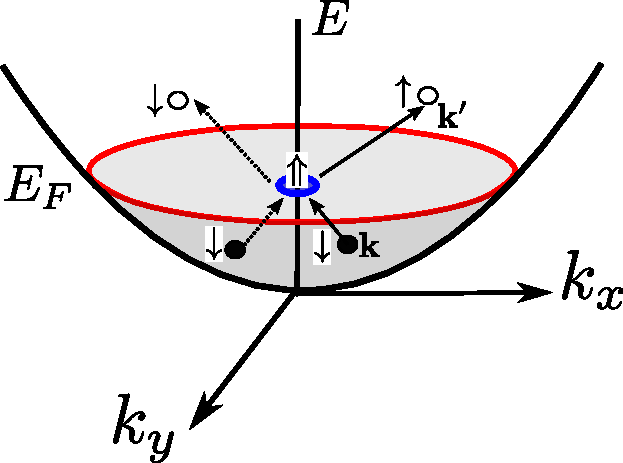
\includegraphics[scale=1]{kondoSetup.pdf}
\caption{The Kondo model is composed of a two-dimensional conduction electron bath (Fermi liquid) coupled to a magnetic impurity via a spin-flip (solid) / non spin-flip (dashed) scattering coupling.}
\end{figure}
\begin{figure}
\centering
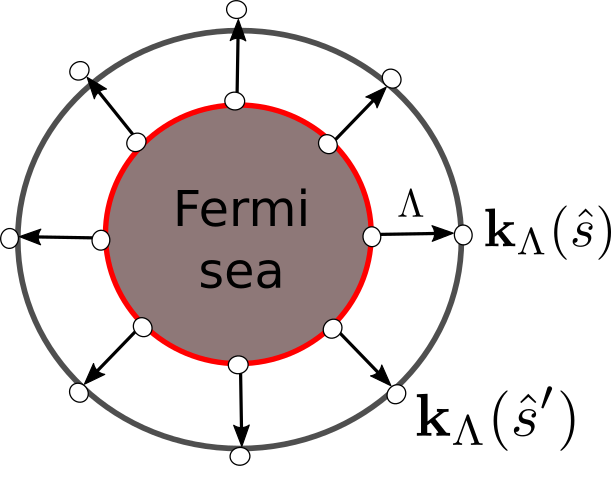
\includegraphics[scale=0.5]{2dKondoTN.png}
\caption{Fermi surface geometry for a circular Fermi volume of non-interacting electrons in 2 spatial dimensions.}
\label{FSgeom}
\end{figure}
%\begin{figure}
%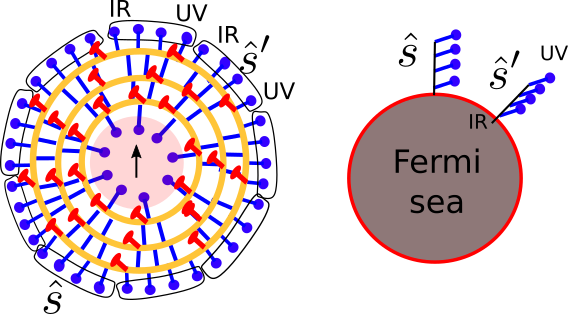
\includegraphics[width=0.7\textwidth]{TNKondo.png}
%\caption{Circular Fermi sea (FS, red circle) of the 2D conduction electron bath, with the arrows representing the different normal directions of the FS. The white circles are electronic states on the curves isogeometric to the FS.}\label{FSgeom}
%\end{figure}
\par\noindent
The $\Lambda$'s are arranged as follows: $\Lambda_{N}>\Lambda_{N-1}>\ldots>0$, where the electronic states farthest from FS $\Lambda_{N}$ are disentangled first, eventually scaling towards the FS. This leads to the Hamiltonian flow equation
\begin{equation}
\centering
H_{(j-1)}=U_{(j)}H_{(j)}U^{\dagger}_{(j)}~,
\end{equation}
where the unitary operation $U_{(j)}$ is the unitary map at RG step $j$. $U_{(j)}$ disentangles all the electronic states 
%$\mathbf{k}_{\Lambda_{j}\hat{s}_{m}},\sigma$ 
$|\mathbf{k}_{\Lambda_{j}\hat{s}_{m}},\sigma\rangle$
on the isogeometric curve and has the form\cite{anirbanmotti}
\begin{equation}
\centering U_{(j)}=\prod_{l}U_{j,l}, U_{j,l}=\frac{1}{\sqrt{2}}[1+\eta_{j,l}-\eta^{\dagger}_{j,l}]~,
\end{equation}
where $\eta_{j,l}$ are electron-hole transition operators following the algebra
\begin{equation}
\lbrace\eta_{j,l},\eta_{j,l}^{\dagger}\rbrace=1~,~\left[\eta_{j,l},\eta_{j,l}^{\dagger}\right]=1~.
\end{equation}
The transition operator can be represented in terms of the diagonal ($H^{D}$) and off-diagonal ($H^{X}$) parts of the Hamiltonian as follows 
\begin{eqnarray}
\eta_{j,l}&=&Tr_{j,l}(c^{\dagger}_{j,l}H_{j,l})c_{j,l}\frac{1}{\hat{\omega}_{j,l}-Tr_{j,l}(H_{j,l}^{D}\hat{n}_{j,l})\hat{n}_{j,l}}~.~~\label{e-TransOp}
\end{eqnarray}
We note that in the numerator of the expression for $\eta_{j,l}$, the operator $Tr_{j,l}(c^{\dagger}_{j,l}H_{j,l})c_{j,l}+h.c.$ is composed of all possible scattering vertices that modify the configuration of the electronic state $|j,l\rangle$. The generic forms of $H^{D}_{j,l}$ and $H^{X}_{j,l}$ are as follows
\begin{eqnarray}
H^{D}_{j,l}&=&\sum_{\Lambda\hat{s},\sigma}\epsilon^{j,l}\hat{n}_{\mathbf{k}_{\Lambda\hat{s}},\sigma}+\sum_{\alpha}\Gamma_{\alpha}^{4,(j,l)}\hat{n}_{\mathbf{k}\sigma}\hat{n}_{\mathbf{k}'\sigma'}+\sum_{\beta}\Gamma_{\beta}^{8,(j,l)}\hat{n}_{\mathbf{k}\sigma}\hat{n}_{\mathbf{k}'\sigma'}(1-\hat{n}_{\mathbf{k}''\sigma''})+\ldots~,\nonumber\\
H^{X}_{j,l}&=&\sum_{\alpha}\Gamma_{\alpha}^{2}c^{\dagger}_{\mathbf{k}\sigma}c_{\mathbf{k}'\sigma'}+\sum_{\beta}\Gamma_{\beta}^{2}c^{\dagger}_{\mathbf{k}\sigma}c^{\dagger}_{\mathbf{k}'\sigma'}c_{\mathbf{k}_{1}'\sigma_{1}'}c_{\mathbf{k}_{1}\sigma_{1}}+\ldots~.
\end{eqnarray}
The operator $\hat{\omega}_{j,l}$ accounts for the quantum fluctuations arising from the non-commutativity between different parts of the renormalized Hamiltonian and has the following form~\cite{anirbanurg1}
\begin{eqnarray}
\hat{\omega}_{j,l}&=&H^{D}_{j,l}+H^{X}_{j,l}-H^{X}_{j,l-1}~.\label{qfOp}
\end{eqnarray}
Upon disentangling electronic states $\hat{s},\sigma$ along a isogeometric curve at distance $\Lambda_{j}$, the following effective Hamiltonian $H_{j,l}$ is generated 
\begin{eqnarray}
H_{j,l}=\prod_{m=1}^{l}U_{j,m}H_{(j)}[\prod_{m=1}^{l}U_{j,l}]^{\dagger}~.
\end{eqnarray}
We note that $H_{j,2n_{j}+1}=H_{(j-1)}$ is the Hamiltonian obtained after disentangling all the electronic states on the isogeometric curve $j$. Below we depict the different terms generated upon successive disentanglement of the states $|\mathbf{k}_{\Lambda_{j}\hat{s}_{l}},\sigma\rangle$ on a given curve,
\begin{eqnarray}
H_{j,l+1}&=&Tr_{j,l}(H_{(j,l)})+\lbrace c^{\dagger}_{j,l}Tr_{j,l}(H_{(j,l)}c_{j,l}),\eta_{j,l}\rbrace\tau_{j,l}, \tau_{j,l}=\hat{n}_{j,l}-\frac{1}{2}\nonumber\\ 
H_{j,l+2}&=&Tr_{j,l+1}(Tr_{j,l}(H_{(j,l)}))+Tr_{j,l+1}(\lbrace c^{\dagger}_{j,l}Tr_{j,l}(H_{(j,l)}c_{j,l}),\eta_{j,l}\rbrace\tau_{j,l})\nonumber\\
&+&\lbrace c^{\dagger}_{j,l+1}Tr_{j,l+1}(Tr_{j,l}(H_{(j,l)})c_{j,l+1}),\eta_{j,l+1}\rbrace\tau_{j,l+1}\nonumber\\
&+&\lbrace c^{\dagger}_{j,l+1}Tr_{j,l+1}(\lbrace c^{\dagger}_{j,l}Tr_{j,l}(H_{(j,l)}c_{j,l}),\eta_{j,l}\rbrace c_{j,l+1}),\eta_{j,l+1}\rbrace\tau_{j,l}\tau_{j,l+1}~.\nonumber\\
H_{j,l+3}&=&\ldots\text{terms with} \tau_{j,l}, \tau_{j,l+1}, \tau_{j,l+2}\ldots\nonumber\\
 &+& \ldots\text{terms with} \tau_{j,l}\tau_{j,l+1}, \tau_{j,l+1}\tau_{j,l+2}, \tau_{j,l}\tau_{j,l+2}\ldots\nonumber\\
 &+&\ldots\text{terms with}\tau_{j,l}\tau_{j,l+1}\tau_{j,l+2}.
\label{2ndDisentanglement}
\end{eqnarray}
Upon disentangling multiple electronic states placed in the tangential direction on a given momentum shell at distance $\Lambda_{j}$ generates RG contribution from leading order scattering processes (terms multiplied with $\tau_{j,l}$, $\tau_{j,l+1}$, etc.) that goes as $Area/Vol=1/L$ and higher order processes like terms multiplied with $\tau_{j,l}\tau_{j,l+1}$ that goes as $(Area)^{2}/Vol^{2}=1/L^{2}$ , $\tau_{j,l}\tau_{j,l+1}\tau_{j,l+2}$ that goes as $(Area)^{3}/Vol^{3}=1/L^{3}$. 
Accounting for only the leading tangential scattering processes, as well as other momentum transfer processes along the normal direction $\hat{s}$, the renormalized Hamiltonian has the form
\begin{eqnarray}
H_{(j-1)}&=&Tr_{j,(1,\ldots,2n_{j})}(H_{(j)})+\sum_{l=1}^{2n_{j}}\lbrace c^{\dagger}_{j,l}Tr_{j,l}(H_{(j)}c_{j,l}),\eta_{j,l}\rbrace\tau_{j,l}~.~~~\label{HRG}
\end{eqnarray}
Here, $2n_{j}$ are the number of electronic states on the isogeometric curve at distance $\Lambda_{j}$, and $\tau_{j,l}= n_{j,l}-\frac{1}{2}$.
%After having disentangled all the electronic states $2n_{j}$ on the isogeometric curve, the effective Hamiltonian $H_{j,2n_{j}+1}=H_{(j-1)}$ is obtained for the next RG step. Disentangling multiple electronic Fock states successively in a given momentum shell at distance $\Lambda_{j}$ from the FS leads to a renormalized contribution from one-particle and higher-particle correlated tangential scattering processes. Accounting for only the leading tangential scattering processes, as well as other momentum transfer processes along the normal direction $\hat{s}$, the renormalized Hamiltonian has the form
%\begin{eqnarray}
%H_{(j-1)}&=&Tr_{j,(1,\ldots,2n_{j})}(H_{(j)})+\sum_{l=1}^{2n_{j}}\lbrace c^{\dagger}_{j,l}Tr_{j,l}(H_{(j)}c_{j,l}),\eta_{j,l}\rbrace\tau_{j,l}~.~~~\label{HRG}
%\end{eqnarray}
%Here, $2n_{j}$ are the number of electronic states on the isogeometric curve at distance $\Lambda_{j}$, and $\tau_{j,l}= n_{j,l}-\frac{1}{2}$.
\section{RG flow to the IR fixed point}\label{fixedPointKondo}
\par\noindent

%The unitary RG process generates the effective Hamiltonian $\hat{H}_{(j-1)}(\omega_{(j)})$ across the various eigendirections $|\Phi(\omega_{(j)})\rangle$ of the $\hat{\omega}_{(j)}$ operator. Note that the associated eigenvalue $\omega_{(j)}$ identifies a sub-spectrum in the interacting many-body eigenspace. The form of $\hat{H}_{(j-1)}(\omega_{(j)})$ is given by
%\begin{eqnarray}
%&&\hat{H}_{(j-1)}(\omega_{(j)}) =\nonumber\\ 
%&&\sum_{j,l,\sigma}\epsilon_{j,l}\hat{n}_{j,l}
%%\nonumber\\&&
%+\frac{J^{(j)}(\omega_{(j)})}{2}\sum_{\substack{j_{1},j_{2}<j-1,\\ m,m'}}\mathbf{S}\cdot c^{\dagger}_{j_{1},\hat{s}_{m},\alpha}\boldsymbol{\sigma}_{\alpha\beta}c_{j_{2},\hat{s}_{m'},\beta}
%%\nonumber\\&&
%(1+
%\sum^{j,2n_{j}}_{j'=N,l=1}\tau_{j',l}+\sum_{j',j''=N,l}^{j}\tau_{j',l}\tau_{j'',l}+\ldots)~.~~~
%\end{eqnarray}
%The renormalization of the effective Hamiltonian within the entangled subspace $\Lambda<\Lambda_{j}$ can be defined as
%\begin{eqnarray}
%\Delta H_{(j)}(\omega_{(j)}) = Tr_{N,\ldots, j}(H_{(j-1)}(\omega_{(j-1)}))-Tr_{N,\ldots, j}(H_{(j)}(\omega_{(j)}))=\sum_{l=1}^{2n_{j}}\lbrace c^{\dagger}_{j,l}Tr_{j,l}(H_{(j)}c_{j,l}),\eta_{j,l}\rbrace~.~~~~
%\end{eqnarray}
%The Hamiltonian renormalization group for the Kondo problem can be observed to generate the RG flow of the Kondo coupling as follows
%\begin{eqnarray}
%\Delta H_{(j)}(\omega)&=&\sum_{\substack{m=1,\\ \beta=\uparrow/\downarrow}}^{n_{j}}\frac{(J^{(j)})^{2}\tau_{j,\hat{s}_{m},\beta}}{2(2\omega\tau_{j,\hat{s}_{m},\beta} - \epsilon_{j,l}\tau_{j,\hat{s}_{m},\beta}-\frac{J^{(j)}}{2}S^{z}(\tau_{j,\hat{s}_{m},\uparrow}-\tau_{j,\hat{s}_{m},\downarrow}))}S^{a}S^{b}\sigma^{a}_{\alpha\beta}\sigma^{b}_{\beta\gamma} c^{\dagger}_{j_{1},\hat{s}_{m},\alpha}c_{j_{2},\hat{s}_{m},\gamma}~,~~~~~~\nonumber\\
%&=&\sum_{\substack{m=1,\\ \beta=\uparrow/\downarrow}}^{n_{j}}\frac{(J^{(j)})^{2}\tau_{j,\hat{s}_{m},\beta}}{2(\omega\tau_{j,\hat{s}_{m},\beta} - \epsilon_{j,l}\tau_{j,\hat{s}_{m},\beta}-\frac{J^{(j)}}{2}S^{z}(\tau_{j,\hat{s}_{m},\uparrow}-\tau_{j,\hat{s}_{m},\downarrow}))}(\frac{3}{4}\delta_{\alpha\gamma}+S^{c}\sigma^{c}_{\alpha\gamma}) c^{\dagger}_{j_{1},\hat{s}_{m},\alpha}c_{j_{2},\hat{s}_{m},\gamma}\nonumber\\
%&=&\sum_{\substack{m=1,\\~\beta=\uparrow/\downarrow}}^{n_{j}}\frac{(J^{(j)})^{2}\tau_{j,\hat{s}_{m},\beta}}{2(2\omega\tau_{j,\hat{s}_{m},\beta}- \epsilon_{j,l}\tau_{j,\hat{s}_{m},\beta}-\frac{J^{(j)}}{2}S^{z}(\tau_{j,\hat{s}_{m},\uparrow}-\tau_{j,\hat{s}_{m},\downarrow}))}\times\nonumber\\
%&\times &\left(\mathbf{S}\cdot c^{\dagger}_{j_{1},\hat{s}_{m},\alpha}\boldsymbol{\sigma}_{\alpha\gamma} c_{j_{2},\hat{s}_{m},\gamma}+\frac{3}{4}c^{\dagger}_{j_{1},\hat{s}_{m},\alpha}c_{j_{2},\hat{s}_{m},\alpha}\right)\nonumber\\
%&=&\frac{1}{2}\sum_{\substack{m=1,\\~\beta=\uparrow/\downarrow}}^{n_{j}}\frac{(J^{(j)})^{2}\left[(\frac{\omega}{2} - \frac{\epsilon_{j,l}}{4})+\frac{J^{(j)}}{2}S^{z}\tau_{j,\hat{s}_{m},\beta}(\tau_{j,\hat{s}_{m},\uparrow}-\tau_{j,\hat{s}_{m},\downarrow}))\right]}{(\omega - \frac{\epsilon_{j,l}}{2})^{2}-\frac{\left(J^{(j)}\right)^{2}}{16}}\times\nonumber\\
%&\times &\left(\mathbf{S}\cdot c^{\dagger}_{j_{1},\hat{s}_{m},\alpha}\boldsymbol{\sigma}_{\alpha\gamma} c_{j_{2},\hat{s}_{m},\gamma}+\frac{3}{4}c^{\dagger}_{j_{1},\hat{s}_{m},\alpha}c_{j_{2},\hat{s}_{m},\alpha}\right)\nonumber\\
%&=&\frac{1}{2}\sum_{m=1}^{n_{j}}\frac{(J^{(j)})^{2}\left[(\omega - \frac{\epsilon_{j,l}}{2})\right]}{(\omega - \frac{\epsilon_{j,l}}{2})^{2}-\frac{\left(J^{(j)}\right)^{2}}{16}}\left(\mathbf{S}\cdot c^{\dagger}_{j_{1},\hat{s}_{m},\alpha}\boldsymbol{\sigma}_{\alpha\gamma}c_{j_{2},\hat{s}_{m},\gamma}+\frac{3}{4}c^{\dagger}_{j_{1},\hat{s}_{m},\alpha}c_{j_{2},\hat{s}_{m},\alpha}+h.c.\right)\label{renH}
%\end{eqnarray}
%In obtaining the above RG equation, we have replaced  $\hat{\omega}_{(j)}=2\omega\tau_{j,\hat{s}_{m},\beta}$. We set the electronic configuration $\tau_{j,\hat{s}_{m},\uparrow}=-\tau_{j,\hat{s}_{m},\downarrow}=\frac{1}{2}$ to account for the spin scattering between the Kondo impurity and the fermionic bath. 
%\par\noindent
%For the sake of completeness, we offer the following clarifications here. The operator $\hat{\omega}_{(j)}$ (eq.\eqref{qfOp}) for RG step $j$ is determined by the occupation number diagonal piece of the Hamiltonian ($H^{D}_{(j-1)}$) attained at the next RG step $j-1$; this demands a self-consistent treatment of the RG equation for $H$ and $\hat{\omega}$ to determine the value of $\omega$. In this fashion, two-particle and higher order quantum fluctuations are automatically encoded into the RG dynamics of the quantum fluctuation operator $\hat{\omega}$. In the present work, however, we restrict our study by ignoring the RG contributions to $\omega$. The electron/hole configuration ($|1_{j,\hat{s}_{m},\beta}\rangle$/$|0_{j,\hat{s}_{m},\beta}\rangle$) of the disentangled electronic state (associated with $\pm \epsilon_{j,l}$ energy) is accounted by the fluctuation energy scales $\pm\omega$. To proceed further, we assume a circular FS such that $\epsilon_{j,l}=\epsilon_{j}-E_{F}\approx\hbar v_{F}\Lambda_{j}$ for $0\leq\Lambda_{j}\leq\Lambda_{0}$. This leads to the RG equation
The unitary RG process generates the effective Hamiltonian's $\hat{H}_{(j)}(\omega)$'s for various eigen directions $|\Phi(\omega)\rangle$
of the $\hat{\omega}$ operator. Note the associated eigenvalue $\omega$ identifies a subspectrum in the interacting many body eigenspace. The form of $\hat{H}_{(j)}(\omega)$ is given by,
\begin{eqnarray}
\hat{H}_{(j)}(\omega) &=& \sum_{j,l,\sigma}\epsilon_{j,l}\hat{n}_{j,l}+\frac{J^{(j)}(\omega)}{2}\sum_{\substack{j_{1},j_{2}<j,\\ m,m'}}\mathbf{S}\cdot c^{\dagger}_{j_{1},\hat{s}_{m},\alpha}\boldsymbol{\sigma}_{\alpha\beta}c_{j_{2},\hat{s}_{m'},\beta}+\sum^{j,n_{j}}_{\substack{a=N,\\ m=1}}J^{(a)}S^{z}s^{z}_{a,\hat{s},m},
\end{eqnarray}
where  $s^{z}_{l,\hat{s},m}=\frac{1}{2}(\hat{n}_{l,\hat{s}_{m},\uparrow}-\hat{n}_{l,\hat{s}_{m},\downarrow})$. The Kondo coupling RG equation for the RG steps(Appendix\ref{Appendix-A}) has the form,
\begin{eqnarray}
\frac{\Delta J^{(j)}(\omega)}{\Delta\log\frac{\Lambda{j}}{\Lambda_{0}}}=\frac{n_{j}(J^{(j)})^{2}\left[(\omega - \frac{\hbar v_{F}\Lambda_{j}}{2})\right]}{(\omega - \frac{\hbar v_{F}\Lambda_{j}}{2})^{2}-\frac{\left(J^{(j)}\right)^{2}}{16}}~,\label{RGeqn}
\end{eqnarray}
where $n_{j}=\sum_{\hat{s}}1$ is the number of states on the isogeometric shell at distance $\Lambda_{j}$ from the Fermi surface. Note that the denominator $\Delta\log\frac{\Lambda{j}}{\Lambda_{0}} =1$ for the RG scale parameterization $\Lambda_{j}=\Lambda_{0}\exp(-j)$. We now redefine Kondo coupling as a dimensionless parameter
\begin{eqnarray}
K^{(j)}=\frac{J^{(j)}}{\omega-\frac{\hbar v_{F}}{2}\Lambda_{j}}~,\label{reparametrization}
\end{eqnarray} 
and operate in the regime $\omega>\frac{\hbar v_{F}}{2}\Lambda_{j}$. 
With the above parametrization of eq.\eqref{reparametrization}, we can convert the difference RG relation (eq.\eqref{RGeqn}) into a continuum RG equation
\begin{eqnarray}
\frac{d K}{d\log\frac{\Lambda}{\Lambda_{0}}}=\left(1-\frac{\omega}{\omega-\hbar v_{F}\Lambda}\right)K+\frac{n(\Lambda)K^{2}}{1-\frac{K^{2}}{16}}
\end{eqnarray}
Upon approaching the Ferm surface $\Lambda_{j}\to 0$,~ $\left(1-\frac{\omega}{\omega-\hbar v_{F}\Lambda}\right)\to 0$ and $n(\Lambda)$ can be replaced by density of states on the Fermi surface $n(0)$:
\begin{eqnarray}
\frac{d K}{d\log\frac{\Lambda}{\Lambda_{0}}}=\frac{n(0)K^{2}}{1-\frac{K^{2}}{16}}
\end{eqnarray}
\begin{figure}[h!]
\centering
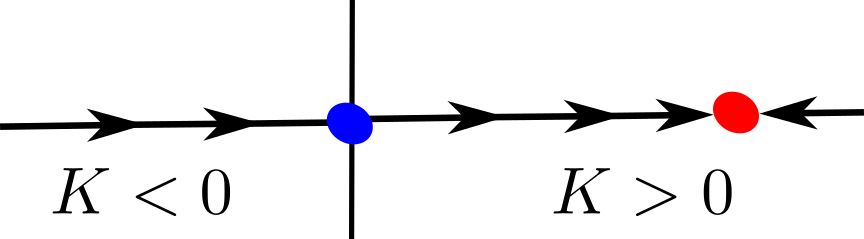
\includegraphics[scale=0.6]{Kondo.png}
\caption{Schematic RG phase diagram for the Kondo problem. The red dot represents intermediate coupling fixed point at $K^{*}=4$ for the case of the AFM Kondo coupling. The blue dot represents the critical fixed point at $K^{*}=0$ for the case of the FM Kondo coupling.} 
\end{figure}
\begin{figure}
\centering
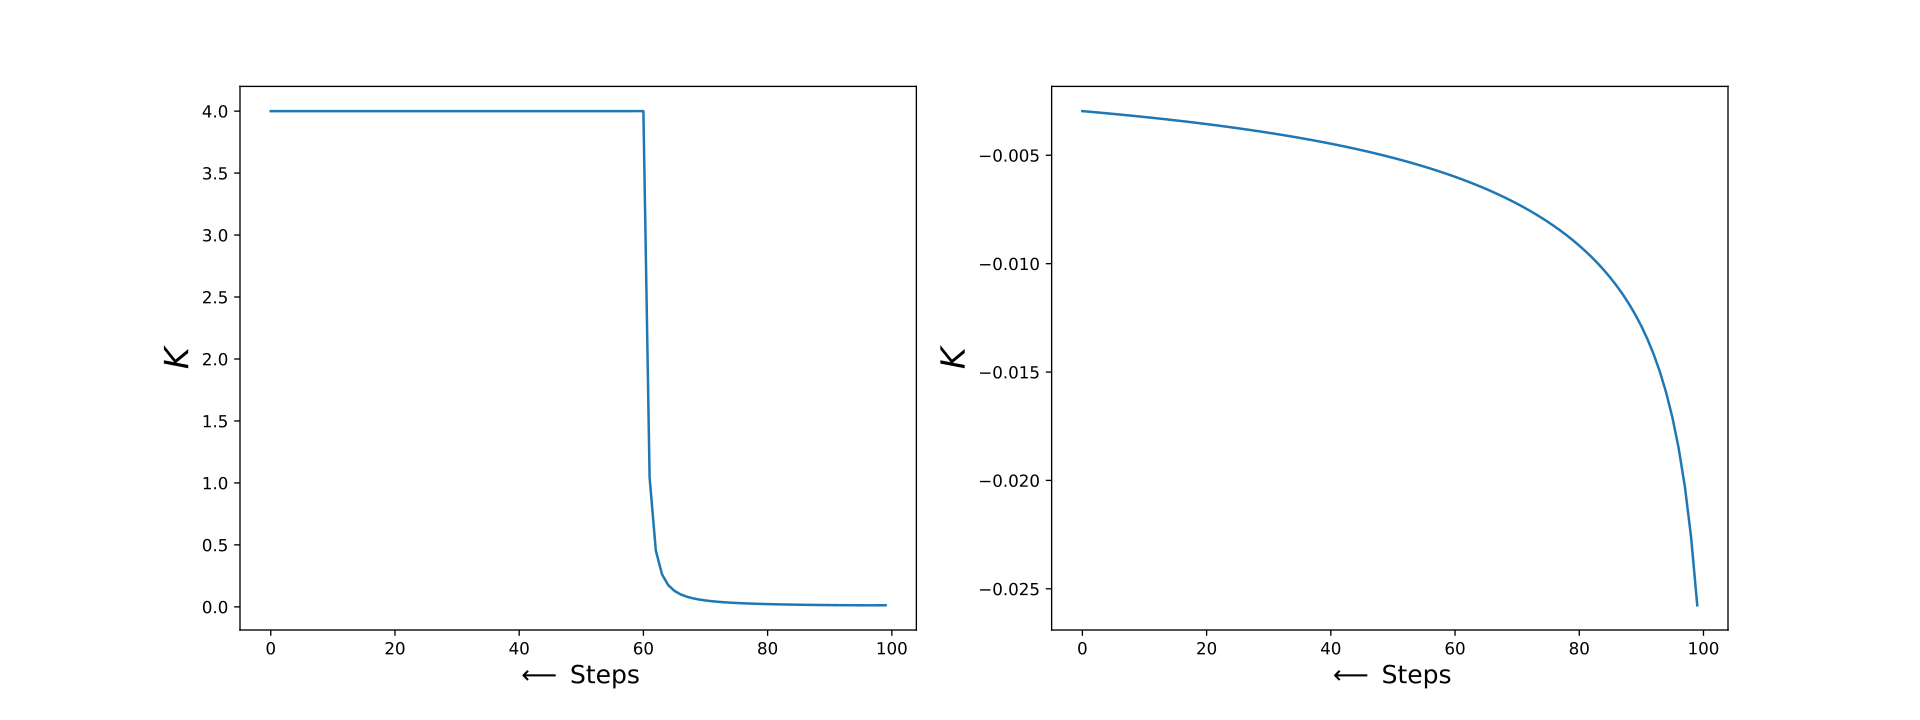
\includegraphics[width=\textwidth]{RG_Flow.png}
\caption{Renormalized dimensionless Kondo coupling $K$ with RG steps ($\log\Lambda_{j}/\Lambda_{0}$)for left panel: $K>0$, and right panel: $K<0$. The growth of the Kondo coupling to a finite value of the intermediate coupling fixed point is evident in the left panel, while the decay to zero at the critical fixed point can be seen in the right panel.} \label{Kondocoupling}
\end{figure}
At this point, we observe an important aspect of the RG equation: for $K<<1$, the RG equation reduces to the one loop form: $\frac{d K}{d\log\frac{\Lambda}{\Lambda_{0}}}=K^{2}$~\cite{anderson1970poor}. On the other hand, the nonperturbative form of the flow equation obtained from the URG formalism shows the presence of intermediate coupling fixed point at $K^{*}=4$ in the antiferromagnetic regime $K>0$. Upon integrating the RG equation and using the fixed point value $K^{*}=4$ we obtain the Kondo energy scale ($T_{K}$) and thence the effective length of the Kondo cloud ($\xi_{K}$)
\begin{eqnarray}
&&\frac{1}{K_{0}}-\frac{1}{2}+\frac{K_{0}}{16}=-n(0)\log\frac{\Lambda^{*}}{\Lambda_{0}}~,\\
&&\Lambda^{*}=\Lambda_{0}\exp\left(\frac{1}{2n(0)}-\frac{1}{n(0)K_{0}}-\frac{K_{0}}{n(0)16}\right)~,\label{gap function}\\
&&T_{K} = \frac{\hbar v_{F}\Lambda^{*}}{k_{B}}= \frac{\hbar v_{F}\Lambda_{0}}{k_{B}}\exp\left(\frac{1}{2n(0)}-\frac{1}{n(0)K_{0}}-\frac{K_{0}}{n(0)16}\right)~,\label{KondoTemp}\\
&&\xi_{K} = \frac{2\pi}{\Lambda^{*}} = \frac{h v_{F}}{k_{B}T_{K}} = \frac{2\pi}{\Lambda_{0}}\exp\left(-\frac{1}{2n(0)}+\frac{1}{n(0)K_{0}}+\frac{K_{0}}{n(0)16}\right)~.\label{KSlength}
\end{eqnarray}
\par\noindent
At the IR fixed point in the AF regime the effective Hamiltonian is given by,
\begin{eqnarray}
H^{*}=\sum_{|\Lambda|<\Lambda^{*}}\hbar v_{F}\Lambda\hat{n}_{\Lambda,\hat{s},\sigma}+\frac{J^{*}}{2}\sum_{\substack{j_{1},j_{2}<j^{*},\\ m,m'}}\mathbf{S}\cdot c^{\dagger}_{j_{1},\hat{s}_{m},\alpha}\boldsymbol{\sigma}_{\alpha\beta}c_{j_{2},\hat{s}_{m'},\beta}+\sum_{j'=N,m=1}^{j^{*},n_{j'}}J^{j'}S^{z}s^{z}_{j',m}~,\label{fixedPointHam}
\end{eqnarray} 
where $m$ refers to the various normal directions $\hat{s}_{m}$ of the Fermi surface. In the above equation, the second term is the effective Hamiltonian for the coupling of the Kondo cloud to the impurity spin, while the third encodes the interaction between the impurity spin moment and the decoupled electronic degrees of freedom that do not belong to the Kondo cloud (lying on radial shells in momentum-space indexed by the RG step $j$). When taken together with the first term (the kinetic energy/dispersion of the lattice conduction electrons), the third gives rise to the local Fermi liquid of Nozieres. In this way, it can be viewed as a (mean-field) self-energy for the decoupled electrons in the $j'$ shell arising from their interaction with the impurity spin
\begin{equation}
\Sigma^{dec}_{j'} = J^{j'}\langle S^{z}\rangle~.  
\end{equation}
As shown in Fig.\ref{Kondocoupling} (left panel), the local nature of the Fermi liquid can be seen by the rapid rise of the coupling $J^{j}=2K_{j}\epsilon_{j}$ with RG step/shell index $j$ only very near to where the Kondo coupling saturates (signalling the Kondo cloud formation). We will see the exact derivation in detail in a subsequent section.
%\par\noindent
%At the IR fixed point in the AF regime, the effective Hamiltonian is given by
%\begin{eqnarray}
%H^{*}=\sum_{|\Lambda|<\Lambda^{*}}\hbar v_{F}\Lambda\hat{n}_{\Lambda,\hat{s},\sigma}+\frac{J^{*}(\omega)}{2}\sum_{\substack{j_{1},j_{2}<j^{*},\\ m,m'}}\mathbf{S}\cdot c^{\dagger}_{j_{1},\hat{s}_{m},\alpha}\boldsymbol{\sigma}_{\alpha\beta}c_{j_{2},\hat{s}_{m'},\beta}
%\end{eqnarray} 
%We can now extract the zero mode from the above Hamiltonian that captures the effective low-energy theory near the Fermi surface
%\begin{eqnarray}
%H_{coll}&=&\frac{1}{N}\sum_{|\Lambda|<\Lambda^{*}}\hbar v_{F}\Lambda\sum_{|\Lambda|<\Lambda^{*}}\hat{n}_{\Lambda,\hat{s},\sigma}+\frac{J^{*}(\omega)}{2}\sum_{\substack{j_{1},j_{2}<j^{*},\\ m,m'}}\mathbf{S}\cdot c^{\dagger}_{j_{1},\hat{s}_{m},\alpha}\boldsymbol{\sigma}_{\alpha\beta}c_{j_{2},\hat{s}_{m'},\beta}\nonumber\\
%		&=&\frac{J^{*}(\omega)}{2}\sum_{\substack{j_{1},j_{2}<j^{*},\\ m,m'}}\mathbf{S}\cdot c^{\dagger}_{j_{1},\hat{s}_{m},\alpha}\boldsymbol{\sigma}_{\alpha\beta}c_{j_{2},\hat{s}_{m'},\beta}~,
%\end{eqnarray}
%where the first term vanishes as the sum over wavevector $\Lambda$ within the symmetric window $\Lambda^{*}$ around the Fermi surface itself vanishes. 
\par\noindent
We can now extract a zero mode from the above Hamiltonian that captures the low energy theory near the Fermi surface,
\begin{eqnarray}
H_{coll}&=&\frac{1}{N}\sum_{|\Lambda|<\Lambda^{*}}\hbar v_{F}\Lambda\sum_{|\Lambda|<\Lambda^{*}}\hat{n}_{\Lambda,\hat{s},\sigma}+\frac{J^{*}}{2}\sum_{\substack{j_{1},j_{2}<j^{*},\\ m,m'}}\mathbf{S}\cdot c^{\dagger}_{j_{1},\hat{s}_{m},\alpha}\boldsymbol{\sigma}_{\alpha\beta}c_{j_{2},\hat{s}_{m'},\beta}+\sum_{j'=N,m=1}^{j,n_{j'}}J^{j'}S^{z}s^{z}_{j',m}\nonumber\\
		&=&\frac{J^{*}}{2}\sum_{\substack{j_{1},j_{2}<j^{*},\\ m,m'}}\mathbf{S}\cdot c^{\dagger}_{j_{1},\hat{s}_{m},\alpha}\boldsymbol{\sigma}_{\alpha\beta}c_{j_{2},\hat{s}_{m'},\beta}+\sum_{j'=N,m=1}^{j^{*},n_{j'}}J^{j'}S^{z}s^{z}_{j',m}~,
\end{eqnarray}
where the first term vanishes as the sum over wavevector $\Lambda$ within the symmetric window $\Lambda^{*}$ around the Fermi surface itself vanishes.
\par\noindent 
Indeed, we observe that the zero mode Hamiltonian at the IR fixed point is responsible for the formation of the Kondo singlet ground state
\begin{equation}
|\Psi*\rangle=\frac{1}{\sqrt{2}}\left[|\uparrow\rangle\sum_{\Lambda,\hat{s}}|1_{\Lambda,\hat{s},\downarrow}\rangle\otimes_{\Lambda'\neq\Lambda,\hat{s}'\neq \hat{s}}|\Lambda',\hat{s}'\rangle-|\downarrow\rangle\sum_{\Lambda,\hat{s}}|1_{\Lambda,\hat{s},\uparrow}\rangle\otimes_{\Lambda'\neq\Lambda,\hat{s}'\neq \hat{s}}|\Lambda',\hat{s}'\rangle\right]~.\label{eigState}
\end{equation}
Note that this state will be in direct product with the wavefunction for the decoupled electronic degrees of freedom.
\subsection{Variation of the Kondo cloud size $\xi_{K}$ and effective Kondo coupling $J^{*}$ as function of bare coupling $J_{0}$}
In Fig.\ref{strong}, we show the variation of the Kondo cloud size $\xi_{K}$ and effective Kondo coupling $J^{*}$ as function of bare coupling $J$ (in units of $t$) in the range $5.7\times 10^{-5}<J<5.4$.
%, intermediate ($1<J<10$) and all the way till the strong coupling regime ($4.9\times 10^{-3}<J<10^{7}$) respectively.
All plots below are obtained for momentum-space grid $100\times 100$ and with RG scale factor $\Lambda_{j}=b\Lambda_{j+1}$ ($b=0.9999 = 1-1/N*N~,~N=100$). The $E_{F}$ for the 2d tight binding band $-W/2<E_{k}=-2t(\cos k_{x}+\cos k_{y})<W/2$ ($W=4t$) is chosen at $E_{F}=-3.9t$, and the bare $k$-space cutoff is set at $\Lambda_{0}\simeq 2.83$. 
%\begin{figure}[ht!]
%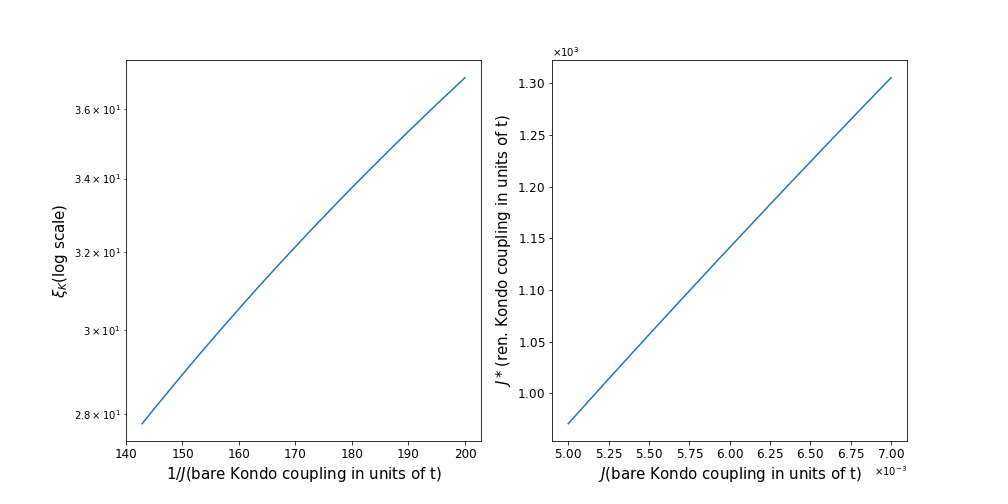
\includegraphics[width=\textwidth]{KondoRegime1.png}
%\caption{Left panel: Kondo cloud length $\xi$ in log scale (y-axis) vs. $1/J_{0}$ (x-axis), right panel: renormalized Kondo coupling $J^{*}$ vs. $J_{0}$, for $5\times 10^{-3}t<J_{0}<7\times 10^{-3}t$.}\label{weak}
%\end{figure}
\par\noindent
The variation of the renormalised Kondo coupling $J^{*}$ with the bare $J$ shown in Fig.\ref{strong} clearly indicates the flow under RG towards saturation at a strong coupling value of $J^{*}_{sat}\sim 16$. Similarly, the variation of the Kondo screening length $\xi_{K}$ with $J$ shows a fall to an asymptotic value of $\xi_{K}\sim 3$ lattice sites at the strong coupling fixed point.
%While the variations of $\xi_{K}$ in the weak and intermediate coupling regimes of $J_{0}$ (Fig. \ref{weak} and \ref{intermediate}) are consistent with the result expected from a 1-loop RG calculation, it clearly shows that $\xi_{K}$ saturates at the final RG step (corresponding to the Kondo cloud formation) at strong coupling (Fig.\ref{strong}). Similarly, $J^{*}$ is consistent with the expectations from a 1-loop RG coupling at weak coupling (Fig.\ref{weak}), shows a tendency towards saturation in the intermediate coupling regime (Fig.\ref{intermediate}) and clearly saturates to a very large (strong coupling) value ($J^{*}_{sat}=1.24\times 10^{4}$, Fig.\ref{strong}) for $10< J_{0}< 10^{7}$. 
We recall that Wilson's NRG calculation for the Kondo problem (for a bath of conduction electrons in the continuum with linear dispersion and a very large UV cutoff $D$) shows that the renormalised Kondo coupling $J^{*}\to\infty$ under flow to strong coupling. This can be reconciled from our URG results by noting that the value of $J^{*}_{sat}$ increases upon rescaling the conduction bath bandwidth $D$ to larger values (by rescaling the nearest neighbour hopping strength $t$). This is shown in Fig.\ref{infinite}, where we see that $J^{*}_{sat}$ increases from a value of $\mathcal{O}(1)$ (in units of $t$) to $\mathcal{O}(10^{9})$ as $t$ is increased from $\mathcal{O}(1)$ to $\mathcal{O}(10^{4})$. Thus, taking the limit of $D\to\infty$ will lead to $J^{*}_{sat}\to\infty$. 
%\begin{figure}[ht!]
%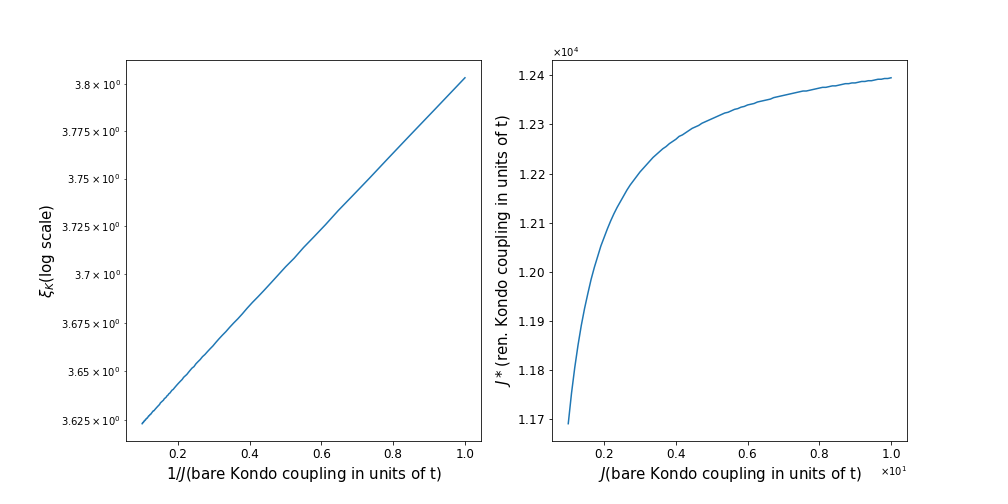
\includegraphics[width=\textwidth]{KondoRegime3.png}
%\caption{Left panel: Kondo cloud length $\xi$ in log scale (y-axis) vs. $1/J_{0}$ (x-axis), right panel: renormalized Kondo coupling $J^{*}$ vs. $J_{0}$, for $t<J_{0}<10t$.}
%\label{intermediate}
%\end{figure}
\begin{figure}[ht!]
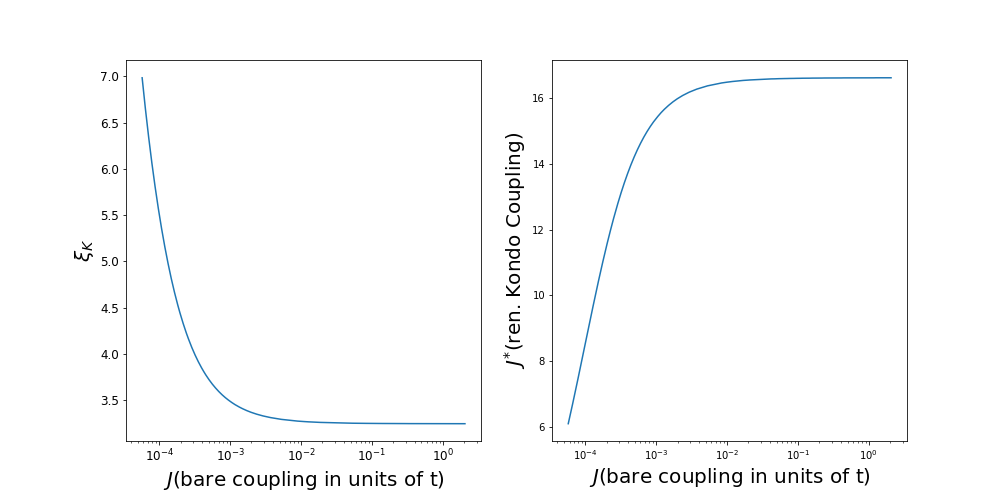
\includegraphics[scale=0.5]{KondoComplete.png}
\caption{Left panel: Kondo cloud length $\xi$ vs. bare Kondo coupling $J$ (x-axis in log scale) in , right panel: renormalized Kondo coupling $J^{*}$ vs. $J$ (x-axis in log scale). The bare Kondo coupling $J$ is chosen to lie within the range $5.7\times 10^{-5}<J<5.4$.}\label{strong}
\end{figure}
\begin{figure}[ht!]
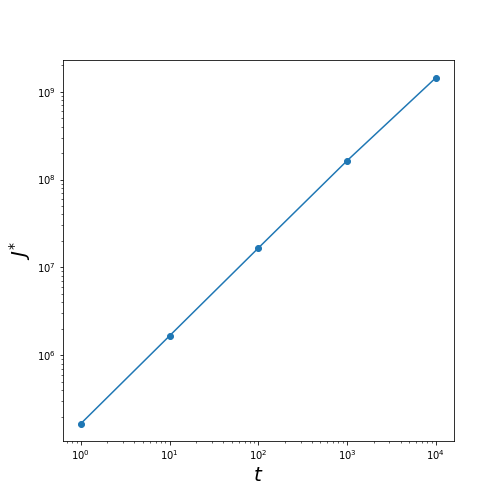
\includegraphics[scale=0.5]{KondoCouplingVst.png}
\caption{Left panel: Variation of the renormalized Kondo coupling $J^{*}$ with the hopping parameter $\mathcal{O}(1)<t<\mathcal{O}(10^{4})$ of the electronic bath (and hence the conduction band width).}\label{infinite}
\end{figure}
\section{Derivation of the local Fermi liquid effective Hamiltonian}\label{localFermi}
We begin by recalling the effective collective Hamiltonian obtained from the URG at the IR fixed point
\begin{eqnarray}
H_{coll}=J^{*}\mathbf{S}\cdot\mathbf{s}+\sum_{l=N,m=1}^{j^{*},n_{l}}J_{l}S^{z}s^{z}_{l,m}
+\sum_{l=N,m=1}^{j^{*},n_{l}}\epsilon_{l}(\hat{n}_{l,m,\uparrow}+\hat{n}_{l,m,\downarrow})
\end{eqnarray}
The thermal density matrix at finite temperatures is then
\begin{eqnarray}
\rho=\exp(-\beta H_{coll})=\prod_{l=N,m=1}^{j^{*},n_{l}}\exp(-\beta\epsilon_{l}(\hat{n}_{l,m,\uparrow}+\hat{n}_{l,m,\downarrow}))\times\exp(-\beta(J^{*}\mathbf{S}\cdot\mathbf{s}+\sum_{l=N,m=1}^{j^{*},n_{l}}J_{l}S^{z}s^{z}_{l,m}))~~~~~
\end{eqnarray}
We now rewrite $H_{coll}$ in the projected basis of the impurity spin and Kondo cloud $(|\uparrow\downarrow\rangle,|\downarrow\uparrow\rangle)$
\begin{eqnarray}
PH_{coll}P &=&\begin{pmatrix}-\frac{J^{*}}{4}+\sum_{l=N,m=1}^{j^{*},n_{l}}\frac{J_{l}}{2}s^{z}_{l,m} & \frac{J^{*}}{2}\\ 
\frac{J^{*}}{2} & -\frac{J^{*}}{4}-\sum_{l=N,m=1}^{j^{*},n_{l}}\frac{J_{l}}{2}s^{z}_{l,m}\end{pmatrix}\nonumber\\
&=&-\frac{J^{*}}{4}+\sigma^{z}h_{z}+\frac{J^{*}}{2}\sigma_{x}=-\frac{J^{*}}{4}+A\boldsymbol{\sigma}\cdot\mathbf{\hat{n}}~,\nonumber\\
 A&=&\sqrt{h^{2}_{z}+\frac{(J^{*})^{2}}{4}}~,~\cos\theta=\frac{h_{z}}{\sqrt{h^{2}_{z}+\frac{(J^{*})^{2}}{4}}}~,~ h_{z}=\sum_{l=N,m=1}^{j^{*},n_{l}}\frac{J_{l}}{2}s^{z}_{l,m}~.
\end{eqnarray}
Thus, the thermal density matrix can be rewritten as
\begin{eqnarray}
&&\rho = \rho_{0}\times \exp(-\beta(J^{*}\mathbf{S}\cdot\mathbf{s}+\sum_{l=N,m=1}^{j^{*},n_{l}}J_{l}S^{z}s^{z}_{l,m}))\nonumber\\
&=&\rho_{0}\times \left [2\exp(-\beta\frac{J^{*}}{4})\cosh\left(\sum_{l=N,m=1}^{j^{*},n_{l}}\frac{\beta J_{l}}{2}s^{z}_{l,m}\right)+\exp(\beta\frac{J^{*}}{4})\exp\left(-\beta A\mathbf{\sigma}\cdot\hat{\mathbf{n}}\right)\right ]\nonumber\\
&=&\rho_{0}\times \left [2\exp(-\beta\frac{J^{*}}{4})\cosh\left(\sum_{l=N,m=1}^{j^{*},n_{l}}\frac{\beta J_{l}}{2}s^{z}_{l,m}\right)+\exp(\beta\frac{J^{*}}{4})\left[\cosh(\beta A)+\boldsymbol{\sigma}\cdot\hat{n}\sinh(\beta A)\right]\right]~,
\end{eqnarray}
where $\rho_{0}= \prod_{l=N,m=1}^{j^{*},n_{l}}\exp(-\beta\epsilon_{l}(\hat{n}_{l,m,\uparrow}+\hat{n}_{l,m,\downarrow}))$ is the thermal density matrix for the disentangled electrons.
\par\noindent
In order to obtain the effective Hamiltonian for just the disentangled electrons, we trace out the impurity and Kondo cloud degrees of freedom from the thermal density matrix ($\rho$)
\begin{eqnarray}
\bar{\rho} &=& Tr_{imp+cloud}(\rho)\nonumber\\
&=&Tr_{imp+cloud}(\rho_{0}\times\exp(-\beta(J^{*}\mathbf{S}\cdot\mathbf{s}+\sum_{l=N,m=1}^{j^{*},n_{l}}J_{l}S^{z}s^{z}_{l,m})))\nonumber\\
&\approx &\rho_{0}\times\exp(\beta\frac{J^{*}}{4})\exp(\beta A)~,~ \text{for}~\beta\to \infty
\end{eqnarray}
Thus, we obtain the effective Hamiltonian for the disentangled electrons
\begin{eqnarray}
H_{eff}=-k_{B}T\log(Tr_{imp+cloud}(\exp(-\beta H^{*}_{K})) &\approx &\sum_{l,m}\epsilon_{l}(\hat{n}_{l,m,\uparrow}+\hat{n}_{l,m,\downarrow})-\frac{J^{*}}{4}-\frac{J^{*}}{2}\sqrt{1+\frac{4h_{z}^{2}}{(J^{*})^{2}}}\nonumber\\
&\approx &\sum_{l,m}\epsilon_{l}(\hat{n}_{l,m,\uparrow}+\hat{n}_{l,m,\downarrow})-\frac{3J^{*}}{4}-\frac{h^{2}_{z}}{J^{*}}~,
\end{eqnarray}
where we recall that $ h_{z}=\sum_{l=N,m=1}^{j^{*},n_{l}}\frac{J_{l}}{2}s^{z}_{l,m}$ contains spin density density interactions between the disentangled electrons of various shells $\Lambda\geq \Lambda^{*}$. Importantly, we see that the ground state energy of the Kondo singlet ($-3J^{*}/4$) appears, signalling that $H_{eff}$ governs the dynamics of quasiparticle excitations.
\par\noindent
Now, upon expanding the square root term within $H_{eff}$ in leading orders of $\frac{h^{z}}{J^{*}}$, we obtain the Fermi liquid fixed point theory
\begin{eqnarray}
H_{FL}=\sum_{l,m}\epsilon_{l}(\hat{n}_{l,m,\uparrow}+\hat{n}_{l,m,\downarrow})-\sum_{l,l',m,m'}f_{ll'}s^{z}_{l,m}s^{z}_{l,m'}, f_{ll'}=\frac{J_{l}J_{l'}}{J^{*}}, s^{z}_{l,m}=\frac{1}{2}(\hat{n}_{l,m,\uparrow}-\hat{n}_{l,m,\downarrow})~.
\end{eqnarray}
Given that the interaction strength $f_{ll'}=\frac{J_{l}J_{l'}}{J^{*}}$ falls off sharply compared to $\epsilon_{\Lambda*}$ with increasing distances $\Lambda>\Lambda^{*}$ (see left panel of Fig.\ref{Kondocoupling}) with the highest magnitude being that  for electronic states on shell $\Lambda^{*}$ ($f_{j^{*}}=J_{*}=4\epsilon_{\Lambda^{*}}$), we obtain the ``local" Fermi liquid Hamiltonian for the disentangled electrons of the shell $\Lambda^{*}$ as
\begin{eqnarray}
H_{LFL}=\epsilon_{*}\sum_{m}(\hat{n}_{*,m,\uparrow}+\hat{n}_{*,m,\downarrow})-J^{*}\sum_{m,m'}s^{z}_{*,m}s^{z}_{*,m'}, s^{z}_{*,m}=\frac{1}{2}(\hat{n}_{\Lambda^{*},m,\uparrow}-\hat{n}_{\Lambda^{*},m,\downarrow})~.
\end{eqnarray}
\subsection{Wilson ratio ($R$) for the local Fermi liquid}
By following the steps shown in Refs.\cite{nozieres1974fermi,coleman2015}, we now obtain the Wilson ratio for the local Fermi liquid we have derived above. For this, we note that the energy cost for quasiparticle excitations with density $\delta n_{*,m,\sigma}$ is given by
\begin{eqnarray}
\mathcal{E}=\mathcal{E}_{0}+\epsilon_{*}\sum_{m,\sigma}\delta n_{*,m,\sigma}+\frac{J^{*}}{4}\sum_{m,m',\sigma}\delta n_{*,m,\sigma}\delta n_{*,m',-\sigma}+\frac{J^{*}}{4}\sum_{m,m',\sigma}n_{*,m,\sigma}\delta n_{*,m',-\sigma}~.
\end{eqnarray}
Then, it is easily seen that 
\begin{eqnarray}
\frac{\delta\mathcal{E}}{\delta n_{*,m,\sigma}}&=&\epsilon_{*}+\frac{J^{*}}{4}\sum_{m'}\delta n_{*,m',-\sigma}+\frac{J^{*}}{4}\sum_{m'}n_{*,m',-\sigma}~,\nonumber\\
&=&\epsilon_{*}+\frac{\Delta\epsilon}{\pi}\delta_{\sigma}(\lbrace n_{*,m',-\sigma}\rbrace,\epsilon_{*})~,
\end{eqnarray}
where we have taken
\begin{eqnarray}
E_{k}-E_{F}&=&-2t\cos(k_{Fx}+\Lambda^{*})-2t\cos(k_{Fy}+\Lambda^{*})+2t\cos k_{Fx}+2t\cos k_{Fy}\nonumber\\
&=&2t(\sin k_{Fx}+\sin k_{Fy})\Lambda^{*}\approx 2t(k_{Fx}+k_{Fy})\Lambda^{*}~.
\end{eqnarray}
Therefore, we obtain
\begin{eqnarray}
\frac{\Delta E}{\Delta \Lambda^{*}}&=&2t(k_{Fx}+k_{Fy})~,~
%\end{eqnarray}%\begin{eqnarray}
\Delta \epsilon=2t(k_{Fx}+k_{Fy})\frac{\pi}{L}~.
\end{eqnarray}
This leads to the quasiparticle (Friedel's) scattering phase shift 
\begin{eqnarray}
\delta_{\sigma}(\lbrace n_{*,m',-\sigma}\rbrace,\epsilon_{*})&=&\frac{\pi J^{*}}{4\Delta\epsilon}\sum_{m'}\delta n_{*,m',-\sigma}+\frac{\pi}{2}+\alpha(\epsilon_{*}-E_{F})~,
\end{eqnarray}
where $\delta_{0}=\frac{\pi}{2}$ is the phase shift accounting for the absorption of an effective single electron (corresponding to the Kondo cloud) into the singlet. The quantity $\alpha(\epsilon^{*}-E_{F})=\frac{\pi J^{*}}{4\Delta\epsilon}\sum_{m'}n_{*,m',-\sigma}-\frac{\pi}{2}$ accounts for the quasiparticle self energy generated by potential scattering with the impurity-cloud singlet~\cite{martin-physrevlett.48.362,nozieres1974fermi,coleman2015}.
Following Ref.\cite{nozieres1974fermi,coleman2015}, we obtain 
%\begin{eqnarray}
%\frac{\delta_{\sigma}(n_{l',m',\sigma'},\epsilon_{l}+\Delta\mu)-\delta_{\sigma}(n_{l',m',\sigma'},\epsilon_{l})}{\Delta\mu}=\frac{\alpha(\epsilon_{l})}{\pi}
%\end{eqnarray}
%Here $\alpha$ is the quasiparticle density of states. In terms of this 
the zero temperature specific heat coefficient (in units of $k_{B}=1$) as
\begin{eqnarray}
\gamma = \frac{2\pi}{3}\alpha(\epsilon_{*}-E_{F})~,
\end{eqnarray} 
and the impurity spin susceptibility as
\begin{eqnarray}
\chi=\frac{4\alpha(\epsilon_{*}-E_{F})}{\pi}~.
\end{eqnarray}
This leads to Wilson's ratio ($R$)
\begin{eqnarray}
R=\frac{\chi}{\gamma}\frac{\pi^{2}}{3}=2~.
\end{eqnarray}
%\section{Impurity spin susceptibility and specific heat calculation for the Kondo Hamiltonian}
%The effective Hamiltonian obtained at the IR fixed point eq.\eqref{fixedPointHam} commutes with the z-component of the net spin vector,
%\begin{eqnarray}
%S^{z}_{tot}=S^{z}+\sum_{\substack{\Lambda,\Lambda'<\Lambda^{*},\\ m,m'\\\alpha,\beta}}c^{\dagger}_{\Lambda,\hat{s}_{m},\alpha}\frac{\sigma_{\alpha\beta}^{z}}{2}c_{\Lambda',\hat{s}_{m'},\beta}+\sum_{\Lambda\geq \Lambda^{*},m}S^{z}s^{z}_{\Lambda,m},~~~ s^{z}_{\Lambda,m}=\frac{1}{2}\left(\hat{n}_{\Lambda,\hat{s}_{m},\uparrow}-\hat{n}_{\Lambda,\hat{s}_{m},\downarrow}\right)~.~~~
%\end{eqnarray}
%\begin{eqnarray}
%[H^{*},S^{z}_{tot}]=0
%\end{eqnarray}
%The spin susceptibility originating purely from the impurity at the IR fixed originating simply from the impurity can be defined as,
%\begin{equation}
%\chi(T)=\frac{1}{kT}\left[\frac{Tr((S^{z}_{tot})^{2}\exp(-H^{*}(0)/kT)}{Tr(\exp(-H^{*}(J^{*})/kT))}-\left(\frac{Tr((S^{z}_{tot})^{2}\exp(-H^{*}(0)/kT)}{Tr(\exp(-H^{*}(J^{*})/kT))}-\frac{1}{4}\right)\right]
%\end{equation}
%Since the eigenvalues of $S^{z}_{tot}$ are good quantum nos for the eigenstates of $H^{*}$ we can use those states to obtain these quantity. Similar thing can be done for the specific heat. The second term in the above expression cancels of the contribution coming to susceptibility from conduction electrons at $J^{*}=0$. The final term $1/4$ cancels of the impurity susceptibility from $J^{*}=0$ term. This prescription is due to Wilson \cite{wilson1975}.
\section{Impurity susceptibility at finite temperatures}\label{susc1}
The complete effective Hamiltonian for the impurity spin ($\mathbf{S}$), Kondo cloud spin ($\mathbf{s}$) and the electrons that comprise the local Fermi liquid has the form,
\begin{eqnarray}
H_{2}=\epsilon_{*}\sum_{m,\sigma}\hat{n}_{*,m,\sigma}+J^{*}\mathbf{S}\cdot\mathbf{s}+J^{*}S^{z}\sum_{m}s^{z}_{*,m}~.
\end{eqnarray}
The Hamiltonian $H_{2}$ has several conserved quantities which we depict below,
\begin{eqnarray}
[H_{2},S^{z}+s^{z}]=0~,~ [H_{2},s^{z}_{*,m}]=0 ~\forall ~1\leq m\leq n_{j}~,
\end{eqnarray}
such that $[H^{*},S^{z}_{tot}]=0$ where $S^{z}_{tot}=S^{z}+s^{z}+\sum_{m}s^{z}_{*,m}$. Therefore, the eigenvalues of $|s^{z}_{*,m}=\uparrow/\downarrow\rangle$  are good quantum numbers; this is simply an outcome of the URG method. We can now extract the effective Kondo impurity-electron cloud Hamiltonian by treating the effect of local Fermi liquid electrons as an effective field $B=J^{*}\sum_{m}\langle s^{z}_{*,m}\rangle$ (note that this the eigenvalue of the LFL spins) on the impurity spin,
\begin{eqnarray}
H^{*}_{K}=J^{*}\mathbf{S}\cdot\mathbf{s}+BS^{z}~.
\end{eqnarray}
%where we have treated the impurity spin density-density interaction ($\sum_{m}J^{*}S^{z}s^{z}_{*,m}$) energy cost $\frac{J^{*}}{4}$ for excitations of the local Fermi liquid lying above the ground state $E_{g}=-\frac{3J^{*}}{4}$. 
It is also important to note that the URG procedure did not lead to the generation of spin density density interaction between the electrons of the Kondo cloud and those of the LFL.
\par\noindent
We now obtain the impurity magnetization and susceptibility from this effective Hamiltonian. The four state eigenspectrum of $H^{*}_{K}$ is given by
\begin{eqnarray}
E_{1}&=&\frac{1}{2}(-\frac{J^{*}}{2}+\sqrt{B^{2}+J^{*2}})~,~E_{2}=\frac{1}{2}(-\frac{J^{*}}{2}-\sqrt{B^{2}+J^{*2}})~,\nonumber\\
E_{3}&=&E_{4}=\frac{J^{*}}{4}~.
\end{eqnarray}
The partition function for this Hamiltonian (with $\beta=\frac{1}{k_{B}T}$) is given by
\begin{eqnarray}
Z(B)=2\exp(\beta\frac{J^{*}}{4})\left[\cosh(\beta\frac{B}{2})+\cosh(\frac{\beta}{2}(\sqrt{B^{2}+J^{*2}}))\right]~.
\end{eqnarray}
The magnetization is then given by,
\begin{eqnarray}
M=\frac{k_{B}T}{Z(B)}\frac{dZ(B)}{dB}=\frac{k_{B}T}{Z(B)}\exp(\beta\frac{J^{*}}{4})\beta\left[\sinh(\beta\frac{B}{2})
+\frac{B}{\sqrt{B^{2}+J^{*2}}}\sinh(\frac{\beta}{2}\sqrt{B^{2}+J^{*2}})\right]~,
\end{eqnarray}
and the susceptibility is obtained by taking the effective field $B\to 0$
\begin{eqnarray}
\chi=\lim_{B\to 0}\frac{dM}{dB}=\frac{\frac{\beta}{4}+\frac{1}{2J^{*}}\sinh(\frac{\beta}{2}J^{*})}{1+\cosh(\frac{\beta}{2}J^{*})}~.
\label{susc}
\end{eqnarray}
\par\noindent
We can now make several important observations based on eq.\ref{susc}. First, the saturation value of $4T_{K}\chi$ as $\beta\to \infty$ (i.e., $T\to 0$) is given by
\begin{eqnarray}
\chi(T=0)=\frac{1}{2J^{*}}~.
\end{eqnarray}
We find that the Wilson number $W=4T_{k}\chi(T=0)=\frac{2T_{k}}{J^{*}}$. For values of $J^{*}\simeq 16.612t$ and $T_{k}\simeq 3.433t$ we obtain $W=0.413$. This is in excellent agreement with the value for $W$ obtained from NRG~\cite{bullaNRGreview} and Bethe Ansatz solution of the Kondo problem~\cite{andreiKondoreview,tsvelickKondoreview}. This is shown in Fig.\ref{suscfig1} (upper panel). Further, we show the variation of $W$ with the bare Kondo coupling $J$ in Fig.\ref{suscfig1} (lower panel). The figure clearly shows the saturation of $W$ to the value mentioned above as $J$ flows to the strong coupling fixed point.
\begin{figure}[ht!]
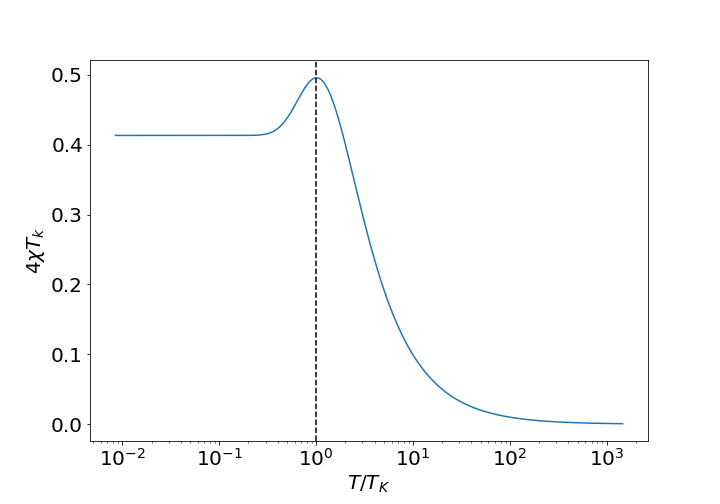
\includegraphics[scale=0.5]{SusceptibilityVsTemp1.png}
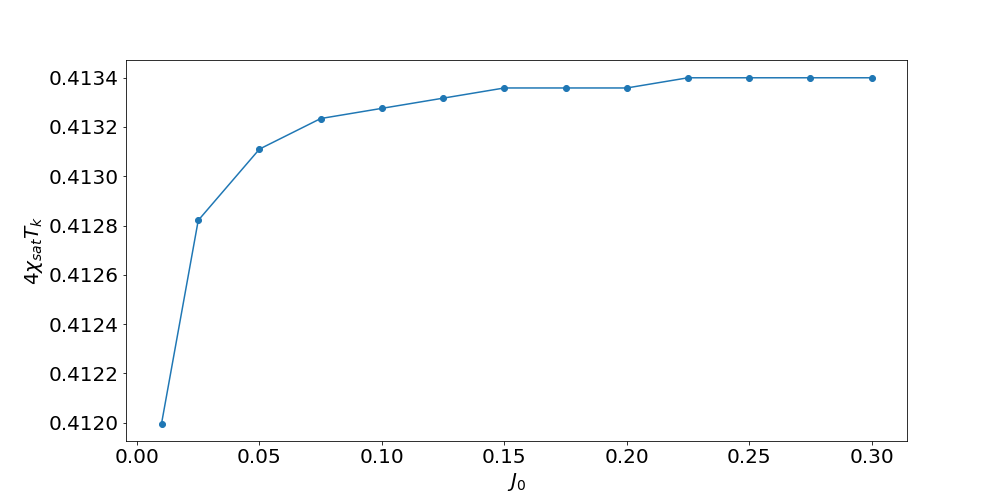
\includegraphics[scale=0.5]{WilsonNumber.png}
\caption{Upper panel: Variation of $4T_{K}\chi$ with $T/T_{K}$. Dashed line shows $T=T_{K}$. Lower panel: Variation of Wilson number $W$ with bare Kondo coupling $J_{0}$. See discussion in text.}\label{suscfig1}
\end{figure}
\par\noindent
Second, the $T_{k}\chi$ vs temperature curve shown in Fig.\ref{suscfig1} has a non-monotonic behaviour, i.e., we find a maxima obtained from the transcendental equation 
\begin{eqnarray}
\frac{d\chi}{d\beta}&=&\frac{1}{4}-\frac{1}{4}\frac{(1+\frac{2}{J^{*}\beta}\sinh\frac{\beta J^{*}}{2})(\frac{J^{*}\beta}{2}\sinh\frac{\beta J^{*}}{2})}{(1+\cosh\beta\frac{J^{*}}{2})^{2}}\nonumber\\ 
\implies (1+\cosh\beta\frac{J^{*}}{2})^{2}&=&\frac{J^{*}\beta}{2}\sinh\frac{\beta J^{*}}{2}+\sinh^{2}\frac{\beta J^{*}}{2}~.~~~~~
\end{eqnarray} 
We confirm from our numerical studies that the temperature ($T_{max}$) corresponding to the maximum value of $T_{K}\chi$ varies as $T_{max}\to T_{k}$ as $J$ flows to strong coupling. Further, we find that the maximum value of $T_{K}\chi$ does not vary with the bare $J$ in the range $\mathcal{O}(10^{-5})<J<\mathcal{O}(1)$.
\begin{figure}[ht!]
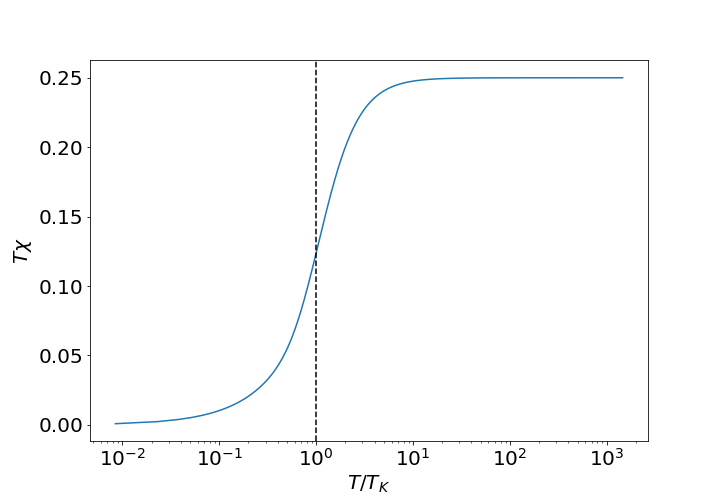
\includegraphics[scale=0.5]{SusceptibilityVsTemp2.png}
\caption{Variation of $T\chi$ with $T/T_{K}$. See discussion in text.}\label{suscfig2}
\end{figure}
\par\noindent
Finally, we find that the saturation value of $T\times\chi$ for $\beta\to 0$ is given by the universal value
\begin{eqnarray}
k_{B}T\chi(T=\infty)=\frac{1}{4}~,
\end{eqnarray}
as shown in Fig.\ref{suscfig2}.
\section{Excitations of the Kondo cloud and the Sommerfield coefficient}\label{susc2}
In this section we will study the effect of the renormalized Kondo coupling on the self energy of the electrons comprising the Kondo cloud. We integrate out the decoupled electronic states to obtain the effective Hamiltonian $H^{*}$ of the impurity + electronic cloud system. In this Hamiltonian we have additionally kept the electronic dispersion to study the effect of electronic density fluctuation due to the inter-electronic interaction mediated by the impurity spin, 
\begin{eqnarray}
H^{*}&=&H_{0}^{*}+\frac{J^{*}}{2}\sum_{\substack{j_{1},j_{2}<j^{*},\\ m,m'}}\mathbf{S}\cdot c^{\dagger}_{j_{1},\hat{s}_{m},\alpha}\boldsymbol{\sigma}_{\alpha\beta}c_{j_{2},\hat{s}_{m'},\beta}\label{effHam}\\
H_{0}^{*}&=&\sum_{|\Lambda_{j}|<\Lambda^{*},\sigma}\epsilon_{j}\hat{n}_{j,\hat{s},\sigma}\label{density}~.
\end{eqnarray}
In order to study the inter-electronic interaction we need to isolate the quantum impurity from the Kondo cloud. This can be done by first recasting the many body eigenstate $|\Psi\rangle$ of $H^{*}$ in the $\uparrow/\downarrow$ basis of the impurity and the associated configuration of the rest electronic states, 
\begin{eqnarray}
|\Psi\rangle = a_{0}|\uparrow_{imp}\rangle|\Phi_{0}\rangle+a_{1}|\downarrow_{imp}\rangle|\Phi_{1}\rangle,\label{decompState}
\end{eqnarray}
here $|\Phi_{0}\rangle$ and $|\Phi_{1}\rangle$ refer to the electronic configurations of the remnant electrons. With the above decomposed state we can rewrite the eigen value relation for $H^{*}_{K}$ as a set of two coupled equations ($E_{1}$ is the eigenvalue),
\begin{eqnarray}
&&a_{0}(H_{0}^{*}+\frac{J^{*}}{2}s_{z})|\Phi_{0}\rangle + a_{1}\frac{J^{*}}{2}s_{+}|\Phi_{1}\rangle = a_{0}E_{1}|\Phi_{0}\rangle\nonumber\\
&&a_{0}\frac{J^{*}}{2}s_{-}|\Phi_{0}\rangle +a_{1}(H_{0}^{*}-\frac{J^{*}}{2}s_{z})|\Phi_{1}\rangle  = a_{1}E_{1}|\Phi_{1}\rangle~.~~~~~
\end{eqnarray}
Combining this two equations we can obtain,
\begin{eqnarray}
&&a_{0}(\frac{J^{*}}{2}s_{z})|\Phi_{0}\rangle + s_{+}\frac{\frac{(J^{*})^{2}}{4}}{E+\frac{J^{*}}{2}s_{z}-H_{0}^{*}}s_{-}|\Phi_{0}\rangle = a_{0}(E-H^{*}_{0})|\Phi_{0}\rangle\label{coupled1}
\end{eqnarray}
From here we obtain the form of the effective Hamiltonian accounting for the leading order density-density and off-diagonal four Fermi interaction terms,
\begin{eqnarray}
H_{eff}&=&\frac{J^{*}}{2}s_{z}+s_{+}\frac{\frac{(J^{*})^{2}}{4}}{(E_{1}+\frac{J^{*}}{2}s_{z})(1-\frac{1}{E_{1}+\frac{J^{*}}{2}s_{z}}H^{*}_{0})}s_{-}\nonumber\\
&\approx &\frac{J^{*}}{2}s_{z}+s_{+}\frac{\frac{(J^{*})^{2}}{4}}{E_{1}+\frac{J^{*}}{2}s_{z}}(1+\frac{1}{E_{1}+\frac{J^{*}}{2}s_{z}}H^{*}_{0}+\frac{1}{E+\frac{J^{*}}{2}s_{z}}H^{*}_{0}\frac{1}{E+\frac{J^{*}}{2}s_{z}}H^{*}_{0})s_{-}+O((H_{0}*)^{3})\nonumber\\
&\approx &\frac{J^{*}}{2}s_{z}+s_{+}\frac{\frac{(J^{*})^{2}}{4}}{E+\frac{J^{*}}{2}s_{z}}  s_{-}+ s_{+}\frac{\frac{(J^{*})^{2}}{4}}{(E_{1}+\frac{J^{*}}{2}s_{z})^{2}}H^{*}_{0}s_{-}+s^{+}\frac{\frac{(J^{*})^{2}}{4}}{(E_{1}+\frac{J^{*}}{2}s_{z})^{2}}H^{*}_{0}\frac{1}{E+\frac{J^{*}}{2}s_{z}}H^{*}_{0}s_{-}, ~~~~~\nonumber\\
&\approx &\frac{J^{*}}{2}s_{z}+(\frac{1}{2}+s_{z})\frac{\frac{(J^{*})^{2}}{4}}{E_{1}-\frac{J^{*}}{2}s_{z}}+s_{+}\frac{\frac{(J^{*})^{2}}{4}}{(E_{1}+\frac{J^{*}}{2}s_{z})^{2}}(s_{-}H^{*}_{0}+[H^{*}_{0},s_{-}])+\nonumber\\
&+&s_{+}\frac{\frac{(J^{*})^{2}}{4}}{(E_{1}+\frac{J^{*}}{2}s_{z})^{2}}H^{*}_{0}\frac{1}{E_{1}+\frac{J^{*}}{2}s_{z}}(s_{-}H^{*}_{0}+[H^{*}_{0},s_{-}])~.
\end{eqnarray}
Finally we obtain the effective Hamiltonian upon setting $E_{1}=0$ in the equation above and choosing $s_{z}=\frac{1}{2}$ (this is the spin configuration associated with the wave function eq.\eqref{decompState} in eq.\eqref{coupled1}, from which the effective Hamiltonian is derived),
\begin{equation}
H_{Eff}=-\frac{3J^{*}}{4}+4(H^{*}_{0}+H^{*}_{0}\frac{4}{J^{*}}H^{*}_{0})+\sum_{k_{1},k_{2},k_{3},k_{4}}\frac{4\epsilon_{k}\epsilon_{k_{1}}}{J^{*}}c^{\dagger}_{k_{4}\uparrow}c^{\dagger}_{k\downarrow}c_{k_{2}\downarrow}c_{k_{1}\uparrow}~.\label{eff_Ham_Kondo}
\end{equation}
The first represents the ground state energy of the singlet configuration, second term accounts for the density density correlation (see eqn.\eqref{density}), the third term accounts for the spin fluctuation mediated electron-electron scattering process respectively.
\pin
In order to study the thermodynamic properties of the Fermi liquid we restrict our attention to the density-density terms only, at a later point we will see the effect of non-Fermi liquid corrections due to the off-diagonal terms. From the density terms we obtain the low excitation energy functional accounting for the quasiparticle interaction,
\begin{eqnarray}
E=E_{0}+\sum_{\mathbf{k}_{\Lambda\hat{s}},\Lambda<\Lambda^{*}}\epsilon_{\mathbf{k}}\delta n_{\mathbf{k}\sigma}+\sum_{\mathbf{k},\mathbf{k}'}\frac{4\epsilon_{\mathbf{k}}\epsilon_{\mathbf{k}'}}{J^{*}}\delta n_{\mathbf{k}\sigma}\delta n_{\mathbf{k}'\sigma'}
\end{eqnarray}
This leads to the renormalized one-particle dispersion, where the  self energy term has the following form,
\begin{eqnarray}
\bar{\epsilon}_{\Lambda}=\epsilon_{\Lambda}+\Sigma_{\Lambda} ,\Sigma_{\Lambda}=(\sum_{\Lambda',\hat{s},\sigma'}\frac{4\epsilon_{\Lambda}\epsilon_{\Lambda'}}{J^{*}}\delta n_{\Lambda',\hat{s},\sigma'}) \text{ for }\Lambda<\Lambda^{*}~. 
\end{eqnarray}
Note that as $\Lambda\to 0$ , $\Sigma_{\Lambda}\to 0$. Next we compute the specific heat of the impurity from the Fermi Dirac distribution of the renormalized quasiparticles,
\begin{eqnarray}
C_{imp}&=&C(J^{*})-C(0)\nonumber\\
&=&\sum_{\Lambda,\hat{s},\sigma}\left(\frac{(\bar{\epsilon}_{\Lambda})^{2}\exp(\beta\bar{\epsilon}_{\Lambda})}{(\exp(\beta\bar{\epsilon}_{\Lambda})+1)^{2}}-\frac{(\epsilon_{\Lambda})^{2}\exp(\beta\epsilon_{\Lambda})}{(\exp(\beta\epsilon_{\Lambda})+1)^{2}}\right),
\end{eqnarray}
$C(J^{*})$ is the specific heat for the electronic system with the Kondo impurity and $C(0)$ is the specific heat for the free electronic system without coupling to Kondo Impurity. The specific heat coefficient is given by $\gamma_{imp}=\frac{C_{imp}}{k_{B}T}$. Fig. shows that $\gamma_{imp}T_{k}$ rises from 0 at high temperatures $T>10^{2}T_{K}$ and saturates at a value $\gamma_{imp}(0)T_{K}=0.0519$ for $T<10^{-2}T_{K}$. The Wilson ratio in Fig. obtained from the ratio of the saturation values of the susceptibility and specific heat coefficient saturates to a value $W=\chi(0)/\gamma_{imp}(0)=2.012$ for $T<10^{-2}T_{K}$.

\begin{figure}
(a)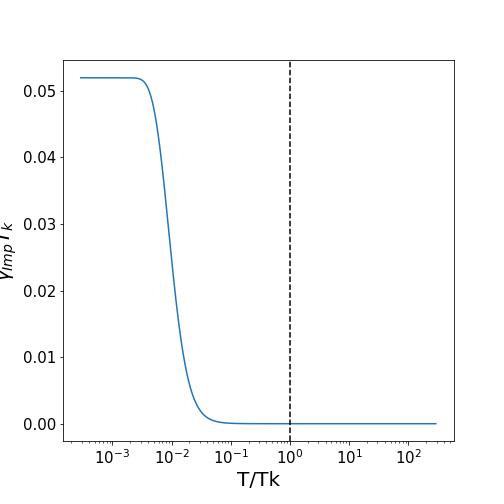
\includegraphics[scale=0.5]{specificHeatCoeff.png}
(b)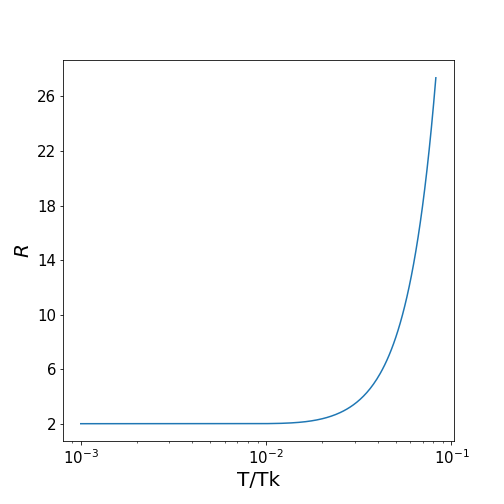
\includegraphics[scale=0.5]{WilsonRatio.png}
\caption{(a)Variation of $\gamma_{imp}T_{K}$ with $T/T_{K}$, dashed line shows $T=T_{k}$. (b)Variation of $R$ Wilson ratio with $T/T_{K}$.}
\end{figure}
\section{Many body correlations and entanglement properties of the Kondo cloud}\label{ent2}
In order to study the effect of the off-diagonal terms  eq.\eqref{eff_Ham_Kondo} on the constituents of the Kondo cloud we perform a reverse URG treatment (shown in Fig.\ref{URGflowScheme}) starting from the Kondo model ground state $|\Psi^{*}\rangle$ at the IR fixed point eq.\eqref{eigState}.
\begin{figure}[!ht]
\centering
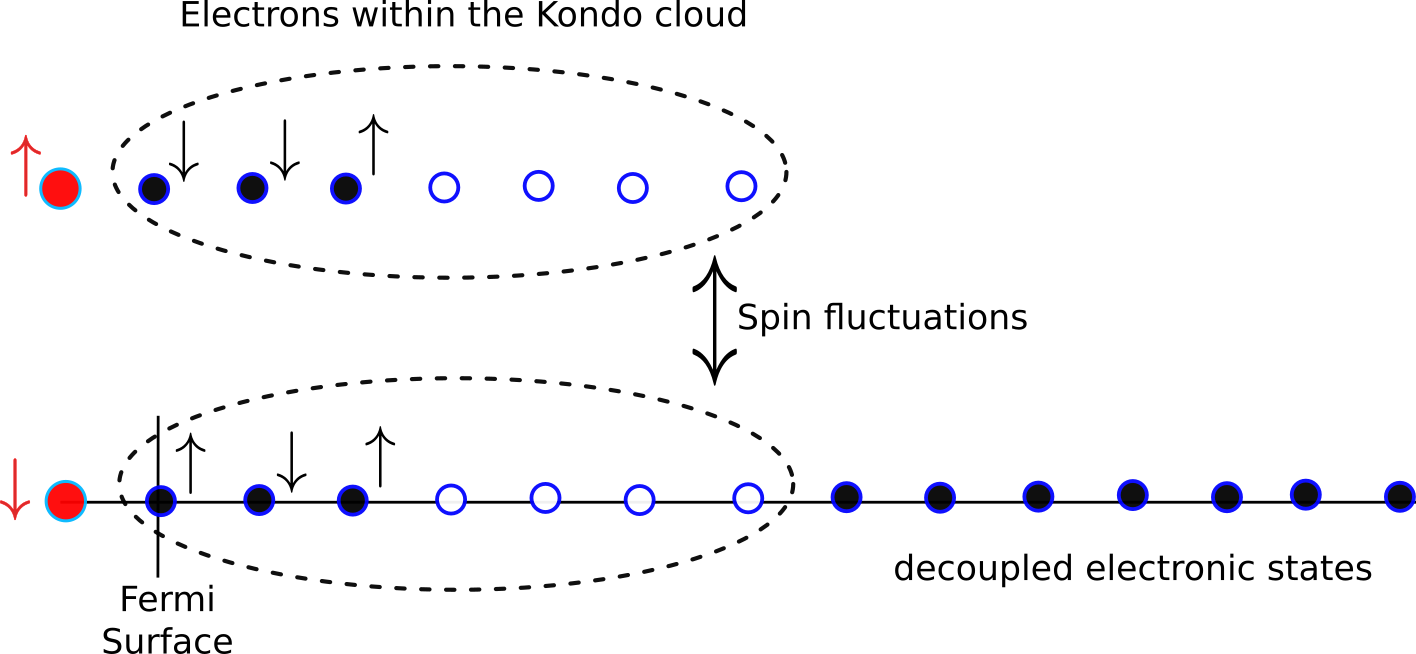
\includegraphics[width=0.7\textwidth]{KC.png}
\caption{Figure describes the electronic Kondo cloud (dashed oval) coupled to the impurity spin(red arrow).}\label{ToyKondo}
\end{figure}
\begin{figure}[!ht]
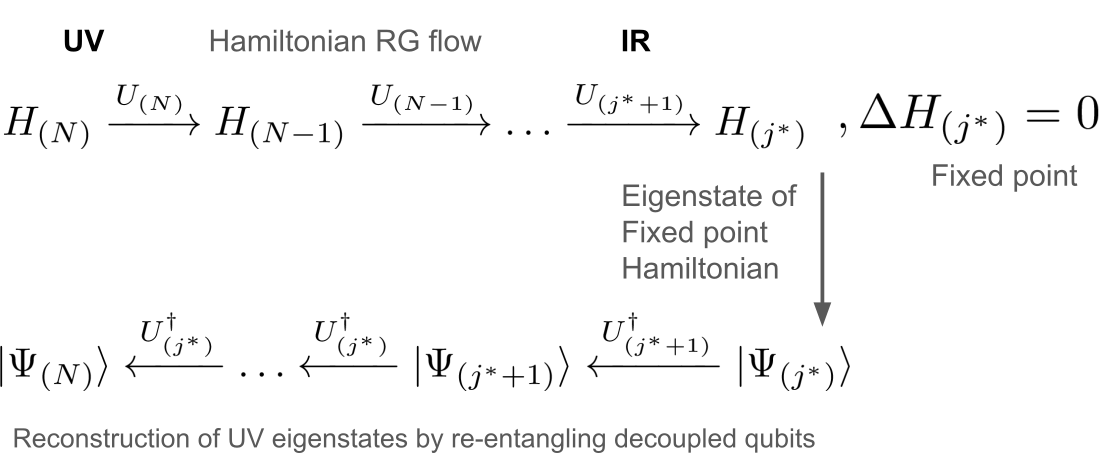
\includegraphics[width=\textwidth]{flowChart.png}
\caption{The first line represent the Hamiltonian RG flow via the unitary maps. Upon reaching the Kondo IR fixed point, reverse RG will re-entangled decoupled electronic states with the Kondo singlet. This will result in generation of the many body eigenstates at UV.}  \label{URGflowScheme}
\end{figure}
\pin
For the present study we take a toy model construction of the ground state wavefunction $|\Psi^{*}\rangle$ eq.\eqref{eigState} at IR, the Kondo impurity couples to $12$ electronic states $|\mathbf{k}\sigma\rangle$ of which three are occupied and 9 are unoccupied. The net spin of the electrons comprising the Kondo cloud is oppositely aligned to that the Kondo impurity. The Kondo cloud system is in tensor product with 14 separable electronic states. This construction is represented in Fig.\ref{ToyKondo} At each URG step $U_{j,\uparrow}U_{j,\downarrow}$ two electronic states $|k_{j},\uparrow\rangle$, $|k_{j\downarrow}\rangle$ are disentangled in reaching the IR fixed point. Upon performing reverse RG at each step two electrons are re-entangled into the eigenstates via the inverse unitary maps $U^{\dagger}_{j,\uparrow}U^{\dagger}_{j,\downarrow}$, Fig.\ref{URGflowScheme}, all total we perform seven reverse RG steps. This reverse RG program is numerically implemented using python. 
\pin
We use the wavefunctions generated under the reverse RG to compute the mutual information between (a) an electron in the Kondo cloud and the impurity electron, and (b) two electrons within the cloud. MI measures the total amount of quantum and classical correlations in a system~\cite{groisman2005}. The mutual information between two electrons is given by 
\begin{eqnarray}\centering
 I(i:j)=-Tr(\rho_{i}\ln\rho_{i})-Tr(\rho_{j}\ln\rho_{j})+Tr(\rho_{ij}\ln\rho_{ij})~,\label{MI}
 \end{eqnarray}
where $\rho_{i}$ or $\rho_{j}$ and $\rho_{ij}$ are the $1$- and $2$-electron reduced density matrices respectively obtained from the wavefunctions obtained at each step of the reverse RG simulation. In Fig.\ref{MI1}, we present the RG flow of both types of mutual information mentioned above. The orange curve in Fig.\ref{MI1}(a) represents the plot for the maximum mutual information $I(e:e)$ (eq.\eqref{MI}) between any two of the electrons comprising the Kondo cloud, and shows that the maximum entanglement content/quantum correlation increases under RG flow from UV to IR. This implies that the electrons within the Kondo cloud is not simply a separable state in momentum space expected of a local Fermi liquid. This is a strong indication of the fact that the two-particle off-diagonal ($c^{\dagger}_{k_{4}\uparrow}c^{\dagger}_{k\downarrow}c_{k_{2}\downarrow}c_{k_{1}\uparrow}$) scattering term in eq.\eqref{eff_Ham_Kondo} is playing a role in the electronic entanglement within the Kondo cloud. Further, the blue curve in Fig.\ref{MI1}(a) shows that the maximum mutual information between the Kondo impurity and any one member of the electronic cloud also increases under RG and to a higher value compared to that between electrons. This originates from the maximally entangled singlet state that is formed between the impurity and the electronic cloud. In this manner, the Kondo impurity mediates the entanglement between electrons (orange curve) in the Kondo cloud.
\pin
In order to understand this further, we also study (i) the maximum density-density correlations $\max_{k,k_{1}}\langle\hat{n}_{k\uparrow}\hat{n}_{k_{1}\downarrow}\rangle$ (blue curve in Fig.\ref{MI1}(b)), and (ii) the maximum two-particle off-diagonal correlations $\max_{k,k_{1}}\langle c^{\dagger}_{k\uparrow}c^{\dagger}_{k_{1}\downarrow}c_{k_{2}\downarrow}c_{k_{3}\uparrow}\rangle$ (orange curve in Fig.\ref{MI1}(b)) between electrons within the Kondo cloud. The plots show clearly that both the correlations grow under RG from UV to IR, finally reach the same value at the IR fixed point. The non-zero values of the off-diagonal correlations reinforce our observation of a non-zero mutual information content between the cloud electrons. This implies that the electronic cloud is, in general, a non-Fermi liquid with non-zero entanglement content. Further studies of the many body entanglement content and transport properties are required to understand the physics of these non-Fermi liquid metal.
\begin{figure}
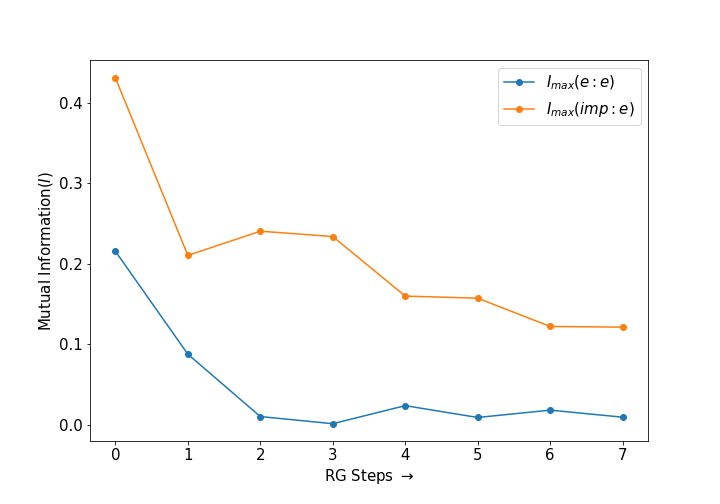
\includegraphics[width=0.7\textwidth]{MIkondo.png}
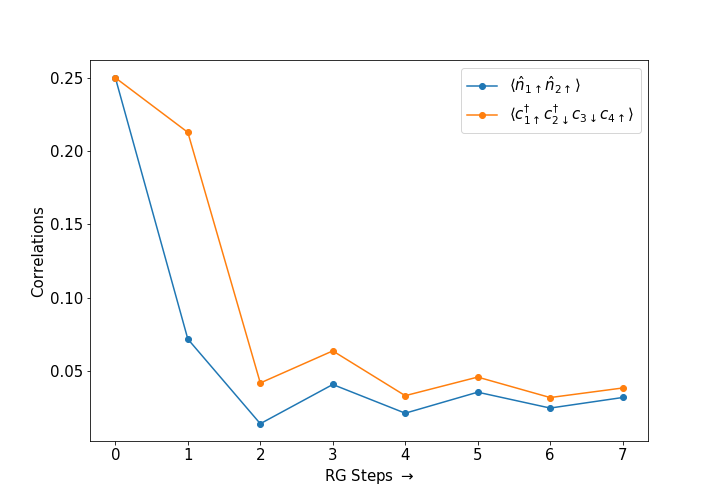
\includegraphics[width=0.7\textwidth]{corrKondo.png}
\caption{Figure(a) shows the RG flows for the maximum mutual information between the impurity and electron (orange curve) and diagonal correlations (blue curve). Figure(b) shows the RG flows for the off-diagonal (orange curve) and diagonal correlations (blue curve).}\label{MI1}
\end{figure}
\section{Conclusion and Future directions}
The Kondo problem~\cite{kondo1964resistance} is one of the oldest and well studied problem of electronic correlations in condensed matter~\cite{anderson1970poor,wilson1975}, and represents a set of benchmarking exercises for verifying the accuracy of the URG method.  The RG analysis of the Kondo Hamiltonian leads to a zero temperature phase diagram revealing a intermediate coupling fixed point for an antiferromagnetic Kondo coupling. At the IR fixed point, we obtained the effective Hamiltonian, the ground state wavefunction and the energy eigenspectrum. This enabled the computation of various  thermodynamic quantities such as the impurity susceptibility, specific heat coefficient, Wilson ratio, Wilson number, all of which  are found to be in excellent agreement with that obtained from the NRG studies~\cite{bullaNRGreview}. 
\pin
Furthermore, we found that the effective Hamiltonian for the Kondo cloud, obtained by integrating out the impurity spin, contains a density-density repulsion (corresponding to the local Fermi liquid) as well as a four-fermion interaction term  description. In order to understand the roles of the two types of electronic correlations better, we performed a comparative study of the RG evolution of four-point number diagonal and number off-diagonal correlators. By using the singlet IR ground state wavefunction obtain from the URG analysis, We also studied the RG evolution of the mutual information (an entanglement based measure) between (a) the impurity and an electron in the cloud and (b) two electrons in the cloud. The results show strong inter-electronic as well as electron-impurity entanglement upon approaching the IR fixed point. This is in agreement with the presence of both types of two-particle correlators at the IR ground state. Indeed, we find that both the number diagonal and number off-diagonal correlators reach same value at the IR fixed point, indicating that the electronic configuration within the Kondo cloud is not simply a local Fermi liquid. 
%Indeed the effective Hamiltonian obtained at the RG fixed point, obtained by integrating out the impurity spin, contains a four-fermion interaction term. 
Future studies needs to be performed for investigating the nature of the correlated metal comprising the Kondo cloud, e.g., various transport observables like  spectral function, resistivity of the electronic system need to be quantified. Such studies should help in providing predictions that can be tested experimentally. 
%\textbf{AM**}
%
%\section{Tensor network representation of the Kondo URG program}
%\par\noindent
%In this section, we present the tensor network representation of the URG program~\cite{anirbanurg1,mukherjee2020}. The yellow blocks represent the complete unitary transformation $U_{(j)}$ for a given RG step composed of individual $U_{j,l}$ unitary operators that disentangle one electronic state $\mathbf{k}_{\Lambda\hat{s}},\sigma$ each. The wavefunction $|\Psi^{*}\rangle$ comprises the IR bulk of the tensor network. The yellow layers are arranged along the RG direction. 
%\begin{figure}
%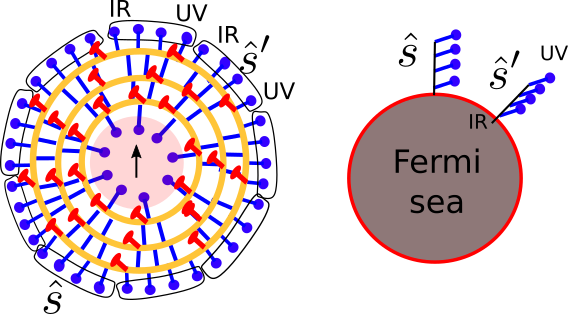
\includegraphics[scale=1]{TNKondo.png}
%\caption{Figure on the left shows a tensor network representation of the Kondo RG with  8 Fermi surface patches. The 32 blue nodes represents the 8 (for 8 $\hat{s}$) sets of 4(along a given normal $\hat{s}$) electronic states (qubits).  arranged from UV to IR (see figure in the right). The yellow circular block represents the unitary gate that disentangles at each RG step 8 electronic qubits at UV. The red nodes represents the disentangled qubits comprising the bulk of the tensor network. At the IR bulk of the tensor network the pink circle represents the Kondo cloud coupling with the spin vector (up arrow).} \label{KondoTN}
%\end{figure}
%\begin{figure}
%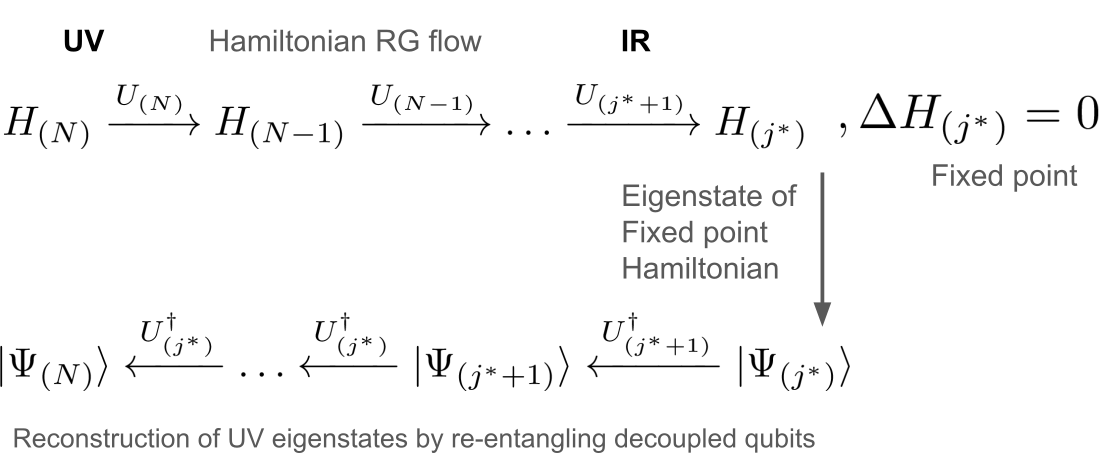
\includegraphics[width=\textwidth]{flowChart.png}
%\caption{The first line represent the Hamiltonian RG flow via the unitary maps. Upon reaching the Kondo IR fixed point, reverse RG will re-entangled decoupled electronic states with the Kondo singlet. This will result in generation of the many body eigenstates at UV.}  \label{eigenUV}
%\end{figure}
%The tensor network Fig.\ref{KondoTN} is composed of yellow layers that lead to a holographic arrangement of eigenstates from UV to IR. As outlined in Fig.\eqref{eigenUV}, by starting from the singlet state obtained at RG fixed point, we can perform the inverse unitary map to regenerate the entanglement with UV degrees of freedom. This enables us in obtaining the complete form of the many-particle wavefunction, and thence the two-point retarded Green's function, along the RG flow direction (RG time) $\tau_{j}=1/v_{F}\Lambda_{j}$
%\begin{eqnarray}
%G(\mathbf{k}\sigma,\tau;\mathbf{k}'\sigma',\tau')=\Theta(\tau-\tau')\langle\Psi_{0}|\lbrace c_{\mathbf{k}\sigma}(\tau)c^{\dagger}_{\mathbf{k}'\sigma'}(\tau')\rbrace|\Psi_{0}\rangle~,
%\end{eqnarray} 
%where $|\Psi_{0}\rangle= U^{\dagger}_{N}\ldots U^{\dagger}_{j^{*}}|\Psi_{(j^{*})}\rangle$ is the many-body state residing at the UV boundary of the tensor network. The many-body rotated $c^{\dagger}$, $c$ operators are given by
%\begin{eqnarray}
%c^{\dagger}_{\mathbf{k}'\sigma'}(\tau')=[U_{j}\ldots U_{N}]c^{\dagger}_{\mathbf{k}'\sigma'}[U_{j}\ldots U_{N}]^{\dagger}~.
%\end{eqnarray}
%From the equal-time Green's function $G(\mathbf{k}\sigma,\tau;\mathbf{k}'\sigma',\tau)$, we can obtain the complete one-particle self-energy. From this, we can compute the spectral function, lifetime, quasiparticle residue etc. Importantly, this quantity is also related to mutual information or entanglement content between a pair of electronic states. This quantity will enable a simultaneous study of the quantum liquid comprising the Kondo cloud from both the many-body and quantum information theoretic perspectives. Indeed, a study of the many-particle entanglement Mott liquid in the 2D Hubbard model at $1/2$-filling has already been carried out using a similar reverse RG formulation~\cite{mukherjee2020}. We now seek to unite this strategy with standard Green's function techniques in the present work.
%
\appendix
\section*{Appendix A: Calculation of effective Hamiltonian from URG}\label{Appendix-A}
\par\noindent
Starting from the Kondo Hamiltonian eq.\eqref{KondoH} and using the URG based Hamiltonian RG equation eq.\eqref{HRG} we obtain,
\begin{eqnarray}
\Delta\hat{H}_{(j)} &=& \sum_{\substack{m=1,\\ \beta=\uparrow/\downarrow}}^{n_{j}}\frac{(J^{(j)})^{2}\tau_{j,\hat{s}_{m},\beta}}{2(2\omega\tau_{j,\hat{s}_{m},\beta} - \epsilon_{j,l}\tau_{j,\hat{s}_{m},\beta}-J^{(j)}S^{z}s^{z}_{j,\hat{s}_{m}})}\nonumber\\
&\times & \bigg[S^{a}S^{b}\sigma^{a}_{\alpha\beta}\sigma^{b}_{\beta\gamma} \sum_{\substack{(j_{1},j_{2}< j),\\ n,o}}c^{\dagger}_{j_{1},\hat{s}_{n},\alpha}c_{j_{2},\hat{s}_{o},\gamma}(1-\hat{n}_{j,\hat{s}_{m},\beta})+S^{b}S^{a}\sigma^{b}_{\beta\gamma}\sigma^{a}_{\alpha\beta} \sum_{\substack{(j_{1},j_{2}<j),\\ n,o}}c_{j_{2},\hat{s}_{o},\gamma}c^{\dagger}_{j_{1},\hat{s}_{n},\alpha}\hat{n}_{j,\hat{s}_{m},\beta}\bigg]\nonumber\\
&+&\sum_{\substack{m=1,\\ \beta=\uparrow/\downarrow}}^{n_{j}}\frac{(J^{(j)})^{2}}{2(2\omega\tau_{j,\hat{s}_{m},\beta} - \epsilon_{j,l}\tau_{j,\hat{s}_{m},\beta}-J^{(j)}S^{z}s^{z}_{j,\hat{s}_{m}})}\bigg[S^{x}S^{y}\sigma^{x}_{\alpha\beta}\sigma^{y}_{\beta\alpha}c^{\dagger}_{j,\hat{s}_{m},\alpha}c_{j,\hat{s}_{m},\beta}c^{\dagger}_{j,\hat{s}_{m},\beta}c_{j,\hat{s}_{m},\alpha}\nonumber\\
&+&S^{y}S^{x}\sigma^{x}_{\alpha\beta}\sigma^{y}_{\beta\alpha}c^{\dagger}_{j,\hat{s}_{m},\beta}c_{j,\hat{s}_{m},\alpha}c^{\dagger}_{j,\hat{s}_{m},\alpha}c_{j,\hat{s}_{m},\beta}\bigg]
\end{eqnarray}
The first term corresponds to the renormalization of the Kondo coupling and describes the sd-exchange interactions for the entangled degrees of freedom,
\begin{eqnarray}
\Delta H^{1}_{(j)}&=&\sum_{\substack{m=1,\\ \beta=\uparrow/\downarrow}}^{n_{j}}\frac{(J^{(j)})^{2}\tau_{j,\hat{s}_{m},\beta}}{(2\omega\tau_{j,\hat{s}_{m},\beta} - \epsilon_{j,l}\tau_{j,\hat{s}_{m},\beta}-J^{(j)}S^{z}s^{z}_{j,\hat{s}_{m}})}\mathbf{S}\cdot c^{\dagger}_{j,\hat{s}_{m},\alpha}\frac{\boldsymbol{\sigma}_{\alpha\beta}}{2}c_{j,\hat{s}_{m},\beta}\nonumber\\
&=&\frac{1}{2}\sum_{\substack{m=1,\\~\beta=\uparrow/\downarrow}}^{n_{j}}\frac{(J^{(j)})^{2}\left[(\frac{\omega}{2} - \frac{\epsilon_{j,l}}{4})+\frac{J^{(j)}}{2}S^{z}\tau_{j,\hat{s}_{m},\beta}(\tau_{j,\hat{s}_{m},\uparrow}-\tau_{j,\hat{s}_{m},\downarrow}))\right]}{(\omega - \frac{\epsilon_{j,l}}{2})^{2}-\frac{\left(J^{(j)}\right)^{2}}{16}}\nonumber\\
&=&\frac{n_{j}(J^{(j)})^{2}\left[(\omega - \frac{\epsilon_{j}}{2})\right]}{(\omega - \frac{\epsilon_{j,l}}{2})^{2}-\frac{\left(J^{(j)}\right)^{2}}{16}}\mathbf{S}\cdot \sum_{\substack{(j_{1},j_{2}<j),\\ n,o}} c^{\dagger}_{j_{1},\hat{s}_{n},\alpha}\frac{\boldsymbol{\sigma}_{\alpha\gamma}}{2}c_{j_{2},\hat{s}_{o},\gamma}\label{HamRG}
\end{eqnarray}
In obtaining the last step of the calculation we have assumed $\epsilon_{j,l}=\epsilon_{j}$ for a circular Fermi surface geoemetry.
The renormalization of the number diagonal Hamiltonian for the immediately disentangled electronic states $|j,\hat{s}_{m},\sigma\rangle$ has the form,
\begin{eqnarray}
\Delta H^{2}_{(j)}&=&\sum_{\substack{m=1,\\ \beta=\uparrow/\downarrow}}^{n_{j}}\frac{(J^{(j)})^{2}}{(2\omega\tau_{j,\hat{s}_{m},\beta} - \epsilon_{j,l}\tau_{j,\hat{s}_{m},\beta}-J^{(j)}S^{z}s^{z}_{j,\hat{s}_{m}})}\bigg[S^{x}S^{y}\sigma^{x}_{\alpha\beta}\sigma^{y}_{\beta\alpha}c^{\dagger}_{j,\hat{s}_{m},\alpha}c_{j,\hat{s}_{m},\beta}c^{\dagger}_{j,\hat{s}_{m},\beta}c_{j,\hat{s}_{m},\alpha}\nonumber\\
&+&S^{y}S^{x}\sigma^{x}_{\alpha\beta}\sigma^{y}_{\beta\alpha}c^{\dagger}_{j,\hat{s}_{m},\beta}c_{j,\hat{s}_{m},\alpha}c^{\dagger}_{j,\hat{s}_{m},\alpha}c_{j,\hat{s}_{m},\beta}\bigg]\nonumber\\
&=&\sum_{\substack{m=1,\\ \beta=\uparrow/\downarrow}}^{n_{j}}\frac{(J^{(j)})^{2}}{(2\omega\tau_{j,\hat{s}_{m},\beta} - \epsilon_{j,l}\tau_{j,\hat{s}_{m},\beta}-J^{(j)}S^{z}s^{z}_{j,\hat{s}_{m}})}S^{z}\frac{\sigma^{z}_{\alpha\alpha}}{2}\bigg[\hat{n}_{j,\hat{s}_{m},\alpha}(1-\hat{n}_{j,\hat{s}_{m},\beta})-\hat{n}_{j,\hat{s}_{m},\beta}(1-\hat{n}_{j,\hat{s}_{m},\alpha})\bigg]\nonumber\\
&=&\sum_{m=1}^{n_{j}}\frac{(J^{(j)})^{2}}{(2\omega\tau_{j,\hat{s}_{m},\beta} - \epsilon_{j,l}\tau_{j,\hat{s}_{m},\beta}-J^{(j)}S^{z}s^{z}_{j,\hat{s}_{m}})}S^{z}s^{z}_{j,\hat{s}_{m}}
\end{eqnarray}
in the last step we have used $\hat{n}_{j,\hat{s}_{m},\alpha}(1-\hat{n}_{j,\hat{s}_{m},\beta})-\hat{n}_{j,\hat{s}_{m},\beta}(1-\hat{n}_{j,\hat{s}_{m},\alpha})=\hat{n}_{j,\hat{s}_{m},\alpha}-\hat{n}_{j,\hat{s}_{m},\beta}$and the spin density for the state $|j,\hat{s}_{m}\rangle$ is given by $s^{z}_{j,\hat{s}_{m}}=\frac{1}{2}(\hat{n}_{j,\hat{s}_{m},\uparrow}-\hat{n}_{j,\hat{s}_{m},\downarrow})$.
\par\noindent
In obtaining the above RG equation we have replaced  $\hat{\omega}_{(j)}=2\omega\tau_{j,\hat{s}_{m},\beta}$. We set the electronic configuration $\tau_{j,\hat{s}_{m},\uparrow}=+\tau_{j,\hat{s}_{m},\downarrow}=-\frac{1}{2}$ to account for the spin scattering between the Kondo impurity and the fermionic bath.  The operator $\hat{\omega}_{(j)}$ (eq.\eqref{qfOp}) for RG step $j$ is determined by the occupation number diagonal piece of the Hamiltonian  $H^{D}_{(j-1)}$ attained at the next RG step $j-1$, this demands a self consistents treatment of the RG equation to determine the $\omega$. In this fashion two particle and higher order quantum fluctuations autamatically get  encoded into the RG dynamics of $\hat{\omega}$. In the present work we restrict our study by ignoring the RG contribution in $\omega$. The electron/hole configuration ($|1_{j,\hat{s}_{m},\beta}\rangle$/$|0_{j,\hat{s}_{m},\beta}\rangle$)  of the disentangled electronic state and associated with $\pm \epsilon_{j,l}$ energy is accounted by $\pm\omega$ fluctuation energy scales. 
From the above Hamiltonian RG equations eq.\eqref{HamRG} we can obtain the form of the Kondo coupling RG equations,
\begin{eqnarray}
\Delta J^{(j)}=\frac{n_{j}(J^{(j)})^{2}\left[(\frac{\epsilon_{j,l}}{2}-\omega)\right]}{(\frac{\epsilon_{j,l}}{2}-\omega)^{2}-\frac{\left(J^{(j)}\right)^{2}}{16}}~.
\end{eqnarray}



% If you have acknowledgments, this puts in the proper section head.
%\begin{acknowledgments}
% put your acknowledgments here.
%\end{acknowledgments}

% Create the reference section using BibTeX:
\bibliography{netbib}

\end{document}
%
% ****** End of file apstemplate.tex ******

